\documentclass[12pt,a4paper]{article}
\usepackage[left=2cm,right=2cm,top=1.5cm,bottom=1.5cm,a4paper]{geometry}

\usepackage{baskervald}
\usepackage[T1]{fontenc}

\usepackage{amsmath}
\usepackage{amsfonts}
\usepackage{amssymb}
\usepackage{makeidx}
\usepackage{graphicx}

\usepackage{mathrsfs}
\usepackage{mathtools}
\DeclarePairedDelimiter\ceil{\lceil}{\rceil}
\DeclarePairedDelimiter\floor{\lfloor}{\rfloor}

\usepackage{xcolor}
\usepackage{cancel}
\newcommand\crossout[3][black]{\renewcommand\CancelColor{\color{#1}}\cancelto{#2}{#3}}
\newcommand\ncrossout[2][black]{\renewcommand\CancelColor{\color{#1}}\cancel{#2}}

\usepackage{pgfplots}
\pgfplotsset{width=10cm,compat=1.9}

\usepackage{tikz}
\usepackage{soul}

\usepackage{caption}
\usepackage{subcaption}

\usepackage{commath} %absolute value
\usepackage{siunitx} %degree

\usepackage{hyperref}

\usepackage{xcolor}
\usepackage{colortbl}
\usepackage{color}
\usepackage[many]{tcolorbox}
\usepackage{enumerate}
\usepackage{booktabs}
\usepackage{dashrule}
\usepackage{caption}

\usepackage{amsthm}
\usepackage{thmtools}
\newtheorem{theorem}{Theorem}[section]
\newtheorem{corollary}{Corollary}[theorem]
\newtheorem{lemma}[theorem]{Lemma}
\newtheorem{proposition}{Proposition}[section]
\newtheorem{fact}[theorem]{Fact}


\theoremstyle{definition}
\newtheorem{example}{Example}[section]

\theoremstyle{definition}
\newtheorem*{definition}{Definition}
\theoremstyle{definition}
\newtheorem*{notation}{Notation}
\theoremstyle{definition}
\newtheorem*{axiom}{Axiom}

\theoremstyle{remark}
\newtheorem*{remark}{\bf Remark}

\theoremstyle{definition}
\newtheorem*{note}{Note}

\newcommand{\dispsty}{\displaystyle}

\newcommand{\makeline}{\rule{\linewidth}{1pt}}
\newcommand{\makedashline}{\hdashrule[0.5ex]{\linewidth}{0.5pt}{2mm}}
\newcommand{\sol}{\textcolor{magenta}{\bf \textit{Sol.}}\quad}
\newcommand{\eg}{\textcolor{blue}{\bf e.g.\quad }}
\newcommand{\ie}{\text{i.e.}}
\newcommand{\lcm}{\normalfont\text{lcm}}
\newcommand{\Var}{\text{Var}}

\author{Ji Yong-hyeon}
\title{\bf\Huge Probability Theory}

\begin{document}
\maketitle
\tableofcontents

\newpage
\section{Introduction}

\subsection{Introduction}
\begin{minipage}{0.49\textwidth}
	\begin{center}
	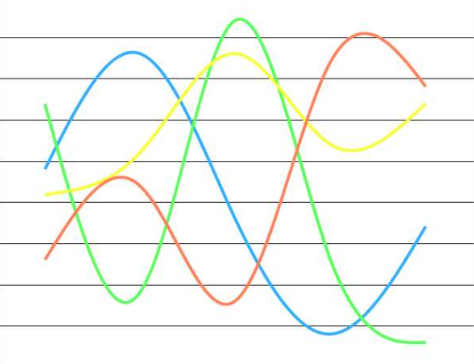
\includegraphics[width=.8\linewidth,height=.13\textheight]{differentiable.png}
	\end{center}
	\begin{itemize}
		\item Continuous and \textbf{Differentiable}
		\item Predictable: Taylor series, \[
		f(x)=\sum_{n=0}^\infty\frac{f^{(n)}(a)}{n!}(x-a)^n.
		\]
		\item \textbf{Deterministic} world
		\item Mathematics of \textbf{\textit{Strong sense}}\begin{itemize}
			\item Definition of \textbf{Function}
		\end{itemize}
		\item Classical mechanics\begin{itemize}
			\item Newtonian mechanics
			\item Law of universal gravitation
		\end{itemize}
	\end{itemize}
\end{minipage}%
\hfill
\begin{minipage}{0.49\textwidth}
	\begin{tabular}{|p{\textwidth}}
		\begin{center}
			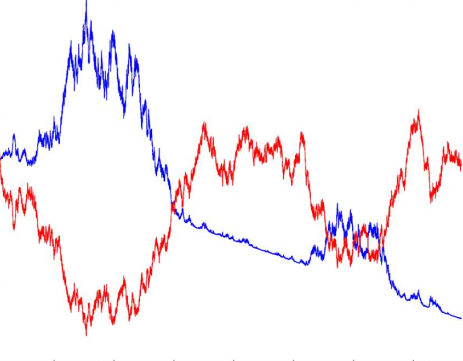
\includegraphics[width=.8\linewidth,height=.13\textheight]{nowhere-differentiable.png}
		\end{center}
		\begin{itemize}
			\item Continuous but \textbf{Nowhere-Differentiable}
			\item \textbf{\textit{Unpredictable}}
			\item[]
			\item[]
			\item \textbf{Non-Deterministic} world
			\item Mathematics of \textbf{\textit{Week sense}}\begin{itemize}
				\item Definition of \textbf{Random variable}
				\item \textbf{Probability Theory}
			\end{itemize}
			\item Quantum mechanics\begin{itemize}
				\item Particle physics
				\item Brownian motion
			\end{itemize}
		\end{itemize}
	\end{tabular}
\end{minipage}%

\subsection{Gambling}
The theory of probability has always been associated with \textbf{gambling}.\begin{itemize}
	\item A \textbf{pair} coin gives you Heads($H$) or Tails($T$) with \textit{equal} probability.
	\item A \textbf{pair} die gives you $1,2,3,4,5$, or $6$ with \textit{equal} probability.
	\item A \textbf{shuffled deck of cards} means that any ordering of cards is \textit{equally likely}.
\end{itemize}
\begin{figure}[h!]
	\centering
	\begin{subfigure}{.3\textwidth}
		\centering
		
\includegraphics[width=.5\linewidth]{coins.png}
	\end{subfigure}%
	\begin{subfigure}{.3\textwidth}
		\centering
		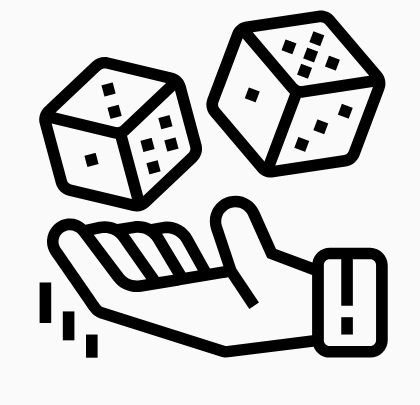
\includegraphics[width=.5\linewidth]{dies.png}
	\end{subfigure}%
	\begin{subfigure}{.3\textwidth}
		\centering
		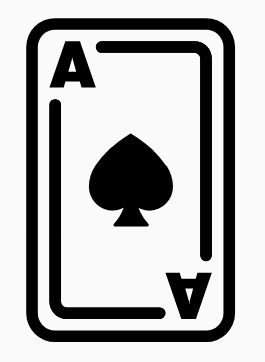
\includegraphics[width=.5\linewidth]{cards.png}
	\end{subfigure}%
\end{figure}\
\newpage
\hypertarget{example1.1}{}\begin{example}\
	\begin{enumerate}
		\item Start with a \textit{shuffled deck of cards} and distribute all 52 cards to 4 player, 13 cards to each. What is the probability that each player gets an Ace?
		\item Next, assume that you are a player and you get a single Ace. What is the probability now that each player gets an Ace?
	\end{enumerate}\ \sol\begin{enumerate}
	\item If any ordering of cards is equally likely, then any position of the four Aces in the deck is also equally likely. There are \[
	\binom{52}{4}=\frac{52!}{4!48!}
	\] possibilities for the positions (slots) for the 4 aces. Out of these, the number of positions that give each player an Ace $13^4$ pick the first slot among the cards that the first player gets, then the second slot among the second player's card, then the third and the fourth slot. Therefore, the answer is \[
	\frac{13^4}{\dispsty\binom{52}{4}}\approx0.1055.
	\] After you see that you have a single Ace, the probability goes up the previous answer need to be divided by the probability that you get a single Ace, which is \[
	\frac{\dispsty13\cdot\binom{39}{3}}{\dispsty\binom{52}{4}}\approx0.4388.
	\] Note that \[
	P(A|B)=\frac{P(A\cap B)}{P(B)}=\frac{P(A)}{P(B)}.
	\] The answer then becomes \[
	\frac{13^4}{13\cdot\dispsty\binom{39}{3}}\approx0.2404.
	\]
\end{enumerate}
\end{example}\

\newpage
\subsection{History of Probability}
\begin{itemize}
	\item \textbf{Blaise Pascal} (1623$\sim$1662)
	\item \textbf{Pierre de Fermat} (1607$\sim$1665)
\end{itemize}
1654 letter from the Flemish aristocrat and notorious gambler Chevalier de M\'{e}r\'{e} to the mathematician and philosopher Blaise Pascal.

\subsection{Equally Likely Outcomes}
\begin{example}
	In a family with 4 children, what is the probability of a 2:2 boy-girl split?\begin{itemize}
		\item One common wrong answer:1/5, as the 5 possibilities for the number of boys are not equally likely. 0:4, 1:3, 2:2, 3:1, 4:0 are not equally likely outcomes.
		\item Another common guess: close to 1, as this is the \textit{most balanced} possibility.
		\item This represents the \textbf{mistaken belief} that symmetry in probabilities should very likely result in symmetry in the outcome.
	\end{itemize}
Let $X=\text{the number of boys}$, then $X\sim\text{Binomial distribution with}\ n=4$, $p=1/2$. Then \[
\Pr[2:2]=P(X=2)=\binom{4}{2}\binom{1}{2}^2\binom{1}{2}^2=\frac{3}{8}.
\]\begin{center}
	\begin{tabular}{|c|ccc|ccc|ccc|ccc|ccc|}
	\toprule
	Outcome && $0:4$ &&& $1:3$ &&& $2:2$ &&& $3:1$ &&& $4:0$ & \\
	\midrule
	Probability && $\dispsty\frac{1}{16}$ &&& $\dispsty\frac{4}{16}$ &&& $\dispsty\frac{6}{16}$ &&& $\dispsty\frac{4}{16}$ &&& $\dispsty\frac{1}{16}$ &\\
	\bottomrule
\end{tabular}
\end{center}
\end{example}\

\subsection{Basic Concepts}
Suppose an experiment is performed, with $n$ possible outcomes comprising a set $S$. Assume also that all outcomes are equally likely. Whether this assumption is \textit{realistic} depends on the context. An \textit{event} $E$ is a set of outcomes, i.e., $E\subset S$. If an event $E$ consists of $m$ different outcomes, then the probability of $E$ is given by \[
P(E)=\frac{m}{n}.
\] The definition of probability only in a \textbf{finite} \textit{sample space} $S$ with equally likely outcomes (Combinatorics).
\begin{example}
	A fair die has 6 outcomes; take $E=\set{2,4,6}$. Then $P(E)=1/2$.
	\begin{itemize}
		\item The most straightforward interpretation is that for a \textit{very large number} of rolls about half of the outcomes will be even.
		\item Note that this requires at least \textbf{the concept of a limit}.
		\item This \textit{relative frequency} interpretation of probability will be explained in detail much later.
	\end{itemize}
\end{example}

\subsection{Problems}
The problem of points, also called the problem of division of the stakes, is a classical problem in probability theory. 

\textbf{Independent trials} resulting in a \textit{success} with probability $p$ and a \textit{failure} with probability $ 1-p $ are performed. What is the probability that $n$ successes occur before $m$ failures? If we think of $A$ and $B$ as playing a game such that $A$ gains 1 point when a success occurs and $B$ gains 1 point when a failure occurs, then the desired probability is the probability that $A$ would win if the game were to be continued in a position where $A$ needed $n$ and $B$ needed $m$ more points to win.


\newpage\section{Combinatorial Analysis}
\subsection{Introduction}
\
\begin{example}
	Toss three fair coins. What is the probability of exactly one Heads (H)?\begin{proof}[\sol]
		There are 8 equally likely outcomes: \[
		S=\set{\text{HHH},\text{HHT},\text{HTH},\text{HTT},\text{TTH},\text{THT},\text{TTH},\text{TTT}}.
		\] Out of these, 3 have exactly one H, that is, \[
		E=\set{\text{HTT},\text{THT},\text{TTH}}\subset S\quad\text{and}\quad P[E]=\frac{3}{8}.
		\]
	\end{proof}
\end{example}
\
\begin{example}
	Let us now compute the probability of a 2:2 boy-girl split in a four-children family. We have 16 outcomes which we will \textit{assume} are equally likely although this is not quite true in reality. We list the outcomes below, although we will soon see that there is a better way.\begin{table}[h!]
		\centering\begin{tabular}{|c|c|c|c|}
			\toprule
			BBBB & BBBG & BBGB & BBGG\\
			\hline
			BGBB & BGBG & BGGB & BGGG\\
			\hline
			GBBB & GBBG & GBGB & GBGG\\
			\hline
			GGBB & GGBG & GGGB & GGGG\\
			\bottomrule
		\end{tabular}
	\end{table}\\ We conclude that \begin{align*}
&P[\text{2:2 split}]=\frac{6}{16}=\frac{3}{8},\\
&P[\text{1:3 split or 3:1 split}]=\frac{8}{16}=\frac{1}{2},\\
&P[\text{4:0 split or 0:4 split}]=\frac{2}{16}=\frac{1}{8}.
\end{align*}
\end{example}
\
\begin{example}
	Roll two dice. What is the most likely sum?
	\begin{proof}[\sol]
		Outcomes are ordered pairs $(i,j), 1\leq i\leq6, 1\leq j\leq 6$.\\
		\\
		\begin{minipage}{0.49\textwidth}
			\centering
			\begin{tabular}{c|c}
				Sum & No. of outcomes\\
				\hline
				2&1\\3&2\\4&3\\5&4\\6&5\\ \cellcolor{-red}7&\cellcolor{-red}6\\
				8&5\\9&4\\10&3\\11&2\\12&1
			\end{tabular}
		\end{minipage}
	\begin{minipage}{0.49\textwidth}
		Let $S=\set{(i,j):1\leq i,j\leq 6}$ then $\#(S)=36$. And \begin{align*}
		E_7&=\set{(i,j):i+j=7}\\
		&=\set{(1,6),(2,5),(3,4),(4,3),(5,2),(6,1)}\subset S.
		\end{align*} Thus, \[
		P[E_7]=\frac{\#(E_7)}{\#(S)}=\frac{6}{36}=\frac{1}{6}.
		\]
	\end{minipage}\\
	\\
	Therefore, our answer is 7, and $P[\text{sum}=7]=6/36=1/6$.
	\end{proof}
\end{example}

\newpage
\subsection{The Basic Principle of Counting}
\textit{How to count?}\\
\\
Listing all outcomes is very inefficient, especially if their number is \textit{large}. We will, therefore, learn a trivial, but conceptually important fact.
\\
\begin{tcolorbox}[colback=white]
	\textbf{The basic principle of counting}\\
	\\
	If an experiment consists of two stages and the first stage	has $m$ outcomes, while the second stage has $n$ outcomes \hl{\textit{regardless of the outcome at the first stage}}, then the
	experiment as a whole has $mn$ outcomes.
\end{tcolorbox}
\
\begin{example}
	Roll a die 4 times. What is the probability that you get different numbers?\begin{proof}[\sol]
		First, we set the sample space $S$ as follows: \[
		S=\set{(a,b,c,d):a,b,c,d\in\set{1,2,3,4,5,6}}.
		\]Let $E$ be the event of different numbers then \[
		E=\set{(a,b,c,d):a\neq b\neq c\neq d}\subset S.
		\], so \[
		P(E)=\frac{\abs{E}}{\abs{S}}=\frac{6\cdot5\cdot4\cdot3}{6\cdot6\cdot6\cdot6}=\frac{5}{18}\ (\approx0.2778).
		\]
	\end{proof}
\end{example}
\
\begin{example}
	Let us now compute probabilities for de M\'{e}r\'{e}'s games. In Game 1, there are 4 rolls and he wins with at least one $6$. The number of good events is $6^4-5^4$, as the number of \textit{bad} events is $5^4$. Therefore \[
	P(\text{win})=1-\left(\frac{5}{6}\right)^4\approx0.5177>\frac{1}{2}.
	\] In Game 2, there are $24$ rolls of two dice and he wins by at least one pair of $6$'s rolled. The number of outcomes is $36^{24}$, the number of bad one is $35^{24}$, thus number of good outcomes equals $36^{24}-35^{24}$. Therefore \[
	P(\text{win})=1-\left(\frac{35}{36}\right)^{24}\approx0.4914<\frac{1}{2}.
	\]\par Chevalier de M\'{e}r\'{e} overcounted the good outcomes in both cases. His count $4\cdot 6^3$ in Game 1 selects a die with a $6$ and arbitrary numbers for other dice. However, may outcomes have more than one six and are hence counted more than once.
\end{example}

\newpage
\subsection{Permutations}

\begin{tcolorbox}[colback=white]
	Assume you have $n$ object. The number of ways to fill $n$ ordered slots with them is \[
	n\cdot(n-1)\cdots2\cdot1=n!,
	\] while the number of ways to fill $k\leq n$ ordered slot is \[
	n\cdot(n-1)\cdots(n-k+1)=\frac{n!}{(n-k)!}.
	\]
\end{tcolorbox}
\
\begin{example}
	Shuffle a deck of cards.\begin{itemize}
		\item $\dispsty P[\text{top card is an Ace}]=\frac{4\cdot51!}{52!}=\frac{1}{13}$.
		\item $\dispsty P[\text{all cards of the same suit end up next to each other}]=\frac{4!\cdot(13!)^4}{52!}\approx4.5\times10^{-28}$.
		\item $\dispsty P[\text{heart are together}]=\frac{(39+1)!\cdot13!}{52!}=\frac{40!\cdot13!}{52!}=6\cdot10^{-11}$.
	\end{itemize}
\end{example}
\
\begin{tcolorbox}[colback=white]
\begin{itemize}
	\item Random choice is made, this mean that \textit{all available choices are \hl{equally likely}}.
	\item \textbf{Statistics (sampling)}\begin{itemize}
		\item \textit{Sampling with replacement} refers to choosing, at random, an object from a population, noting its properties, putting the object back into the population, and then repeating.
		\item Sampling without replacement omits the putting back part.
	\end{itemize}
\end{itemize}
\end{tcolorbox}
\
\begin{example}
	A bag has $6$ pieces of paper, each with one of the letters, $E, E, P, P, P$, and $R$, on it. Pull $6$ pieces at random out of the bag $(1)$ without, and $(2)$ with replacement. What is the probability that these pieces, in order, spell $PEPPER$?\begin{proof}[\sol]
		For sampling without replacement:\begin{enumerate}
			\item An outcome is an ordering of the pieces of paper $E_1E_2P_1P_2P_3R$.
			\item The number of outcomes thus is $6!$.
			\item The number of good outcomes is $3!2!$.
		\end{enumerate} Thus the probability is $\dispsty\frac{3!2!}{6!}$. Another solution is \[
	\frac{3}{6}\times\frac{2}{5}\times\frac{2}{4}\times\frac{1}{3}\times\frac{1}{2}\times1=\frac{3!2!}{6!}.
	\]\\
	\\ For sampling with replacement, the answer is $\dispsty\frac{3^3\cdot2^2}{6^6}=\frac{1}{2\cdot6^3}$ quite a lot smaller.
	\end{proof}
\end{example}
\ \\
\begin{example}
	Sit 3 men and 3 women at random $(1)$ in a row of chairs and $(2)$ around a table. Compute $P[\text{all women sit together}]$, In case $(2)$, also compute $P[\text{men and women alternate}]$.\begin{proof}[\sol]
		In case $(1)$, the answer is $\dispsty\frac{4!3!}{6!}=\frac{1}{5}$. For case $(2)$, pick a man, say John Smith, and sit him first. Then, we reduce to a row problem with $5!$ outcomes; the number of good outcomes is $3!\cdot 3!$. The answer is $\dispsty\frac{3}{10}$.\\
		\\
		For last question, the seats for the men and women are fixed after John Smith takes his seat and so the answer is $\dispsty\frac{3!2!}{5!}=\frac{1}{10}$.
	\end{proof}
\end{example}
\
\begin{example}
	A group consists of $3$ Norwegians, $4$ Swedes, and $5$ Finns, and they sit at random around a table. What is the probability that all groups end up sitting together?\begin{proof}[\sol]
		The answer is $\dispsty\frac{3!4!5!2!}{11!}$.
	\end{proof}
\end{example}

\subsection{Combinations}
\
\begin{tcolorbox}[colback=white]
	Let $\dispsty\binom{n}{k}$ be the number of different subsets with $k$ elements of a set with $n$ elements. Then \begin{align*}
	\binom{n}{k}&=\frac{n(n-1)\cdots(n-k+1)}{k!}\\
	&=\frac{n!}{k!(n-k)!}.
	\end{align*}
\end{tcolorbox} To understand why the above is true, first choose a subset, then order its elements in a row to \hl{fill $k$ ordered slots with elements from the set with $n$ objects}. Then distinct choices of a subset and its ordering will end up as distinct orderings. Therefore, \[
\binom{n}{k}k!=n(n-1)\cdots(n-k+1).
\] $\dispsty\binom{n}{k}$ is called $n$ choose $k$ or binomial coefficient as it appears in the binomial theorem:\begin{tcolorbox}[colback=white]
	 \[(x+y)^n=\sum_{k=0}^n\binom{n}{k}x^ky^{n-k}\]
\end{tcolorbox}\
\\
Also, note that \[
\binom{n}{0}=\binom{n}{n}=0\quad\text{and}\quad\binom{n}{k}=\binom{n}{n-k}.
\]

\subsection{Multinomial Coefficients}
\begin{tcolorbox}[colback=white]
	\begin{notation}
		The number of ways to divide a set of $n$ elements into $r$ (distinguishable) subsets of $n_1,n_2,\cdots,n_r$ elements, where $n_1+\cdots+n_r=n$, is denoted by $\dispsty\binom{n}{n,\cdots, n_r}$ and \begin{align*}
		\binom{n}{n,\cdots, n_r}&=\binom{n}{n_1}\binom{n-n_1}{n_2}\binom{n-n_1-n_2}{n_3}\cdots\binom{n-n_1-\cdots-n_{r-1}}{n_r}\\
		&=\frac{n!}{n_1!n_2!\cdots n_r!}.
		\end{align*}
	\end{notation}
\end{tcolorbox} To understand the slightly confusing word \textit{distinguishable}, just think of painting $n_1$ elements red, then $n_2$ different elements blue, etc. These colors distinguish among the different subsets.
\\
\begin{example}
	A fair coin is tossed $10$ times. What is the probability that we get exactly $5$ Head?\begin{proof}[\sol]
		$P[\text{exactly 5 Heads}]=\binom{10}{5}/2^{10}$ ($\approx0.2461$), as one needs to choose the position of the five heads among 10 slots to fix a good outcome.
	\end{proof}
\end{example}
\
\begin{example}
	We have a bag that contains $100$ balls, $50$ of them red and $50$ blue. Select $5$ balls at random. What is the probability that $3$ are blue and $2$ are red?\begin{proof}[\sol]
		\[
		P[\text{$3$ are blue and $2$ are red}]=\frac{\dispsty\binom{50}{3}\binom{50}{2}}{\dispsty\binom{100}{5}}\ (\approx0.3189).
		\]
	\end{proof}
\end{example}
\
\begin{example}
	Here we return \hyperlink{example1.1}{Example 1.1} and solve it more slowly. Shuffle a standard deck of 52 cards and deal 13 cards to each of the 4 players. What is the probability that each player gets and Ace?\begin{proof}[\sol]
		The first way uses an outcomes to be an ordering of 52 cards:\begin{enumerate}
			\item There are $52!$ equally likely outcomes.
			\item Let us first 13 cards go to the first player, the second 13 cards to the second player, etc. Pick a slot within each of the our segments of $13$ slots for an Ace. There are $13^4$ possibilities to choose these four slots for the Aces.
			\item The number of choices to fill these four positions with (four different) Aces is $4!$
			\item Order the rest of the cards in $48!$ ways.
		\end{enumerate} The probability, then, is $\dispsty\frac{13^44!48!}{52!}(\approx0.1055)$.\\
	\\
	The second way, via a small leap of faith, assumes that each set of the our \textit{positions of the four Aces} among the $52$ shuffled cards is equally likely. You may choose to believe this intuitive fact or try to write down a formal proof: the number of permutations that result in a given set $F$ of four positions is independent of $F$. Then: \begin{enumerate}
		\item The outcomes are the positions of the $4$ Aces among the $52$ slots for the shuffled cards of the deck.
		\item The number of outcomes is $\dispsty\binom{52}{4}$.
		\item The number of good outcomes is $13^4$, as we need to choose one slot among $13$ cards that go to the first player, etc.
	\end{enumerate} The probability, then ,is $\dispsty\frac{\dispsty13^4}{\dispsty\binom{52}{4}}$ which agrees with the number we obtained the first way.\\
\\
Let us also compute $P[\text{one person has al l four Aces}]$. Doing the problem the second way, we get\begin{enumerate}
	\item The number of outcomes is $\dispsty\binom{52}{4}$.
	\item To fix a good outcomes, pick one player($\binom{4}{1}$ choices) and pick four slots for the Aces for that player ($\binom{13}{4}$ choices).
\end{enumerate} The answer, then, is\[
\frac{\dispsty\binom{4}{1}\binom{13}{4}}{\dispsty\binom{52}{4}}(\approx0.0106)
\] a slot smaller then the probability of each player getting.
	\end{proof}
\end{example}
\
\begin{example}
	Roll a die $12$ times. What is the $P[\text{each number appers exactly twice}]$?
	\begin{proof}[\sol]\
		\begin{enumerate}
			\item An outcomes consists of filling each of the $12$ slots (for the $12$ rolls) with an integer between $1$ and $6$ (the outcomes of the roll).
			\item The number of outcomes, therefore, is $6^12$.
			\item To fix a good outcome, pick two slots for $1$, then pick two slots for $2$, with $\dispsty\binom{12}{2}\binom{10}{2}\cdots\binom{2}{2}$ choices.
		\end{enumerate} The probability, then, is $\dispsty\frac{\binom{12}{2}\binom{10}{2}\cdots\binom{2}{2}}{6^{12}}$.\\
	\\
	Another question: what is the $P[1\text{ appears exactly}\ 3\ \text{times},\ 2\ \text{appears exactly}\ 2\ \text{times} ]$?\\
	\\ To fix a good outcomes now, pick three slots for $1$, two slots for $2$, and fill the remaining $7$ slots by numbers $3,\cdots,6$. The number of choices is $\binom{12}{3}\binom{9}{2}4^7$.
	\end{proof}
\end{example}
\newpage
\begin{example}
	We have $14$ rooms and $4$ colors, white, blue, green, and yellow. Each room is painted at random with one of the four colors. There are $4^{14}$ equally likely outcomes, so, for example, \[
	P[\text{5 white, 4 blue, 3 green, 2 yellow rooms}]=\frac{\binom{14}{5}\binom{9}{4}\binom{5}{3}\binom{2}{2}}{4^{14}}.
	\]
\end{example}
\begin{example}
	A middle row on a plane seat $7$ people. Three of them order chicken(C) and the remaining four pasta(P). The flight attendant returns with the meals, but has forgotten who ordered what and discovers that they are all asleep, so she puts the meals in front of them at random. what is the probability that all receive correct meals?
	\begin{proof}[\sol]
		A reformulation makes the problem clearer: we are interested in $P[\text{3 people who orderd C get C}]$. Let us label the people $1,\cdots,7$ and assume that $1,2$ and $3$ ordered $C$. The outcome is a selection of $3$ people from the $7$ who receive $C$, the number of them is $\binom{7}{3}$, and there is a \textit{single} good outcomes. So, the answer is $\frac{1}{\binom{7}{3}}=\frac{1}{35}$. Similarly, \begin{align*}
		&P[\text{no one who ordered C get C}]=\frac{\binom{4}{3}}{\binom{7}{3}}=\frac{4}{35},\\
		&P[\text{a single person who ordered C get C}]=\frac{3\cdot\binom{4}{2}}{\binom{7}{3}}=\frac{18}{35},\\
		&P[\text{two persons who ordered C get C}]=\frac{\binom{3}{2}\cdot4}{\binom{7}{3}}=\frac{12}{35}.
		\end{align*}
	\end{proof}
\end{example}

\subsection{Problems}
\begin{enumerate}[\bf 1.]
	\item A California licence plate consists of a sequence of seven symbols: number, letter, letter, letter, number, number, number, where a letter is any one of 26 letters and a number is one among $0,1,\cdots,9$. Assume that all licence plates are equally likely. ($a$) What is the probability that all symbols are different? ($b$) What is the probability that all symbols are different and the first number is the largest among the numbers?\begin{proof}[\sol]
		\ \begin{enumerate}[($a$)]
			\item content...
		\end{enumerate}
	\end{proof}
\end{enumerate}



\newpage
\section{Axioms of Probability}
How can we \textit{mathematically} define a \textit{random experiment}?\\
\\
What we have are \textbf{outcomes} (which tell you exactly what happens), \textbf{events} (sets containing certain outcomes), and \textbf{probability} (which attaches to every event the likelihood that it happens).
\\
\begin{tcolorbox}[colback=white]
	\begin{fact}
		It is not possible to choose a uniform positive integer at random.
	\end{fact}\tcblower\begin{proof}
	Suppose that we have a uniform distribution over the positive integers and that \[0<\varepsilon<1\] is a candidate for the probability of a specific positive integer occurring. Then \begin{align*}
	P\left(\set{1,2,\cdots,\ceil*{\frac{1}{\varepsilon}}+1}\right) &=\varepsilon\left(\ceil*{\frac{1}{\varepsilon}}+1\right)\\
	&\geq\varepsilon\left(\frac{1}{\varepsilon}+1\right)=(1+\varepsilon)\\
	&>1\ (\because\varepsilon\in(0,1)).
	\end{align*} This is a contradiction as \textit{no} probability may be strictly greater than $1$.
\end{proof}
\end{tcolorbox}

\subsection{Sample Space and Events and Axioms of Probability}
A \textit{probability space} is a triple $(\Omega,\mathscr{F},P)$.\begin{itemize}
	\item $\Omega$ is an arbitrary set, representing \textit{the set of outcomes}, sometimes called the \textbf{sample space}.
	\item $\mathscr{F}$($\sigma$-algebra) is a collection of events, \ie, a set of subsets of $\Omega$.\begin{itemize}
		\item An \textbf{event} $A\in\mathscr{F}$ is necessarily a subset of $\Omega$.
		\item $\mathscr{F}$ needs to be a $\sigma$-algebra(measure theory):\begin{enumerate}[(1)]
			\item $\varnothing\in\mathscr{F}$
			\item $A\in\mathscr{F}\implies A^c\in\mathscr{F}$
			\item $A_1,A_2,\cdots\in\mathscr{F}\implies\bigcup_{i=1}^\infty A_i\in\mathscr{F}$.
		\end{enumerate}
		\item We call events $A_1,A_2,\cdots$ are \textbf{pairwise disjoint} if $A_i\cap A_j=\varnothing$ for $i\neq j$.
	\end{itemize}
	\item The probability $P$ is a number attached to every event $A$ and satisfies the following three axioms:
\end{itemize}

\begin{tcolorbox}[colback=white]
	\begin{enumerate}[\bf \text{Axiom} 1.]
		\item For every event $A$, $P(A)\geq0$.
		\item $P(\Omega)=1$.
		\item If $A_1,A_2,\cdots$ is a sequence of pairwise disjoint events, then \[
		P\left(\bigcup_{i=1}^\infty A_i\right)=\lim\limits_{n\to\infty}\sum_{i=1}^nP(A_i)=\sum_{i=1}^\infty P(A_i)\quad(\text{Countable additivity}).
		\]
	\end{enumerate}
\end{tcolorbox}

\newpage
\begin{example}
	For $\Omega=\set{1,2,3,4,5,6}$, \[
	P(A)=\frac{(\text{number of elements in $A$})}{6}.
	\] The random experiment here is rolling a fair die. Clearly, this can be generalized to any finite set with equally likely outcomes.
\end{example}\
\\
\begin{example}
	For $\Omega=\set{1,2,\cdots}=\mathbb{N}$, you have numbers $p_1,p_2,\cdots\geq0$ with $p_1+p_2+\cdots=1$. For any $A\subset\Omega$, \[
	P(A)=\sum_{i\in A}p_i.
	\] For example, toss a fair coin repeatedly until the first Heads. Your outcome is the number of tosses. Here, $p_i=1/2^i$, so \[
	\sum_{i=1}^\infty p_i=\sum_{i=1}^\infty\left(\frac{1}{2}\right)^i=\frac{1/2}{1-1/2}=1.
	\] Note that $p_i$ cannot be chosen to be equal, as you cannot make the sum of infinitely many numbers to be 1: $\forall p_i=p\geq>0$, \[
	\sum_{i=1}^{\infty}p=\lim\limits_{n\to\infty}\sum_{i=1}^np=\lim\limits_{n\to\infty}np=\infty\neq1.
	\]
\end{example}\
\\
\begin{example}
	Pick a point from inside the unit circle centered at the origin. Here $\Omega=\set{x,y}:x^2+y^2<1$ and \[
	P(A)=\frac{\text{Area($A$)}}{\text{Area($\Omega$)}}=\frac{\text{Area($A$)}}{\pi}.
	\]\begin{figure}[h!]
		\centering
		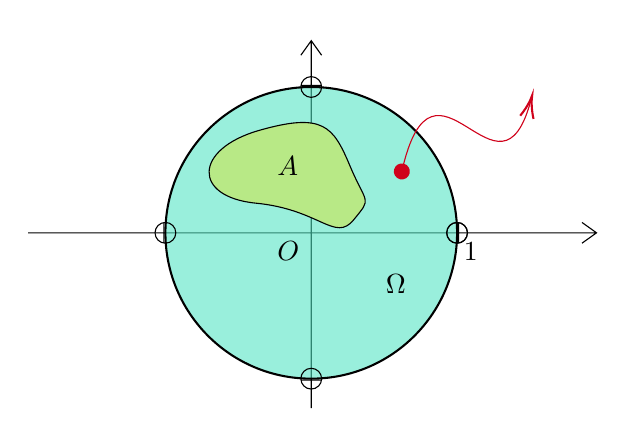
\begin{tikzpicture}[x=0.75pt,y=0.75pt,yscale=-1,xscale=1]
		%uncomment if require: \path (0,300); %set diagram left start at 0, and has height of 300
		
		%Shape: Axis 2D [id:dp6266538637785948] 
		\draw  (223,154.57) -- (496.8,154.57)(359.35,62) -- (359.35,239) (489.8,149.57) -- (496.8,154.57) -- (489.8,159.57) (354.35,69) -- (359.35,62) -- (364.35,69) (430.35,149.57) -- (430.35,159.57)(288.35,149.57) -- (288.35,159.57)(354.35,83.57) -- (364.35,83.57)(354.35,225.57) -- (364.35,225.57) ;
		\draw   ;
		%Shape: Circle [id:dp3611798676876232] 
		\draw  [fill={rgb, 255:red, 80; green, 227; blue, 194 }  ,fill opacity=0.58 ][line width=0.75]  (289.09,154.57) .. controls (289.09,115.76) and (320.55,84.31) .. (359.35,84.31) .. controls (398.16,84.31) and (429.62,115.76) .. (429.62,154.57) .. controls (429.62,193.38) and (398.16,224.84) .. (359.35,224.84) .. controls (320.55,224.84) and (289.09,193.38) .. (289.09,154.57) -- cycle ;
		%Shape: Polygon Curved [id:ds2459808067923741] 
		\draw  [fill={rgb, 255:red, 184; green, 233; blue, 134 }  ,fill opacity=1 ] (334,105.3) .. controls (365.2,96.3) and (370,103.3) .. (378,122.3) .. controls (386,141.3) and (388.8,137.3) .. (379.8,148.3) .. controls (370.8,159.3) and (363.6,143.3) .. (332.8,140.3) .. controls (302,137.3) and (302.8,114.3) .. (334,105.3) -- cycle ;
		%Curve Lines [id:da23949104710289637] 
		\draw [color={rgb, 255:red, 208; green, 2; blue, 27 }  ,draw opacity=1 ]   (403,125) .. controls (418.64,56) and (450.16,148.42) .. (465.34,90.11) ;
		\draw [shift={(465.8,88.3)}, rotate = 463.6] [color={rgb, 255:red, 208; green, 2; blue, 27 }  ,draw opacity=1 ][line width=0.75]    (10.93,-3.29) .. controls (6.95,-1.4) and (3.31,-0.3) .. (0,0) .. controls (3.31,0.3) and (6.95,1.4) .. (10.93,3.29)   ;
		\draw [shift={(403,125)}, rotate = 282.77] [color={rgb, 255:red, 208; green, 2; blue, 27 }  ,draw opacity=1 ][fill={rgb, 255:red, 208; green, 2; blue, 27 }  ,fill opacity=1 ][line width=0.75]      (0, 0) circle [x radius= 3.35, y radius= 3.35]   ;
		
		% Text Node
		\draw (394,173.47) node [anchor=north west][inner sep=0.75pt]  [color={rgb, 255:red, 0; green, 0; blue, 0 }  ,opacity=1 ]  {$\Omega $};
		% Text Node
		\draw (341.8,157.4) node [anchor=north west][inner sep=0.75pt]    {$O$};
		% Text Node
		\draw (341.8,116.4) node [anchor=north west][inner sep=0.75pt]    {$A$};
		% Text Node
		\draw (431.62,157.97) node [anchor=north west][inner sep=0.75pt]    {$1$};
		
		\draw   (429.62, 154.57) circle [x radius= 5, y radius= 5]   ;
		\draw   (429.62, 154.57) circle [x radius= 5, y radius= 5]   ;
		\draw   (289.09, 154.57) circle [x radius= 5, y radius= 5]   ;
		\draw   (359.35, 84.31) circle [x radius= 5, y radius= 5]   ;
		\draw   (359.35, 224.84) circle [x radius= 5, y radius= 5]   ;
		\end{tikzpicture}
	\caption{}
\end{figure} It is important to observe that if $A$ is singleton (a set whole element is a single point) then $P(A)=0$. This means that we cannot attach the probability to outcomes---you hit a single point (or even a line) with probability 0, but a ``fatter'' set with positive area you hit with positive probability.
\end{example}

\newpage
\subsection{Some Simple Properties}
\textbf{Consequences of the axioms:}\begin{enumerate}[(C1)]
	\item[(C0)] $P(\varnothing)=0$.\begin{proof}
		For $A_1=A_2=\cdots=\varnothing$, by \textbf{Axiom 3}, \[
		P(\phi)=P(\varnothing\cup\varnothing\cup\cdots)=P\left(\bigcup_{i=1}^\infty A_i\right)=\lim\limits_{n\to\infty}\sum_{i=1}^nP(A_i)=\lim\limits_{n\to\infty}\sum_{i=1}^nP(\varnothing)=\lim\limits_{n\to\infty}nP(\phi).
		\] Suppose that $P(\phi)\neq 0$. Then $P(\phi)=\lim\limits_{n\to\infty}nP(\phi)=\infty$. It is contradiction. Hence $P(\phi)=0$.
	\end{proof}
	\item If $A_1\cap A_2=\varnothing$, then $P(A_1\cup A_2)=P(A_1)+P(A_2)$.\begin{proof}
		Let $A_i=\varnothing$ for $i\geq3$. Suppose $A_\cap A_2=\varnothing$. Then, by \textbf{Axiom 3},
		\begin{align*}
		P(A_1\cup A_2)&=P(A_1\cup A_2\cup\varnothing\cup\varnothing\cup\cdots)\\&=P(A_1\cup A_2\cup A_3\cup A_4\cup\cdots)\\
		&=P\left(\bigcup_{i=1}^\infty A_i\right)=\lim\limits_{n\to\infty}\sum_{i=1}^nP(A_i)\\
		&=\lim\limits_{n\to\infty}\left(\sum_{i=1}^2P(A_i)+\sum_{i=3}^nP(A_i)\right)\\
		&=\sum_{i=1}^2P(A_i)+\crossout[red]{0}{\lim\limits_{n\to\infty}\sum_{i=3}^nP(A_i)}\\
		&=P(A_1)+P(A_2).
		\end{align*}
	\end{proof}
	\item $P(A^c)=1-P(A)$.\begin{proof}
		Apply to (C1) to $A_1=A, A_2=A^c$. Then \[
		P(\Omega)=P(A\cup A^c)=P(A)+P(A^c)=1.
		\]
	\end{proof}
	\item $0\leq P(A)\leq 1$.\begin{proof}
		By \textbf{Axiom 1}, $0\leq P(A)$. Using that $P(A^c)\geq 0$ in (C2), \[
		P(A^c)=1-P(A)\geq0\implies P(A)\leq 1.
		\]
	\end{proof}
	\item If $A\subset B$, $P(B)=P(A)+P(B\setminus A)\geq P(A)$.\begin{proof}
		Using (C1) for $A_1=A$ and $A_2=B\setminus A$, \[
		P(B)=P(A)+P(B\setminus A)
		\] and since $P(B\setminus A)\geq 0$ by \textbf{Axiom 1}, $P(B)\geq P(A)$.
	\end{proof}
	\item $P(A\cup B)=P(A)+P(B)-P(A\cap B)$.\begin{proof}
		Let $P(A\setminus B)=p_1$, $P(A\cap B)=p_{12}$, and $P(B\setminus A)=p_2$. Note that $A\setminus B, A\cap B$, and $B\setminus A$ are pairwise disjoint. Then $P(A)=p_1+p_{12}$, $P(B)=p_2+p_{12}$, and $P(A\cup B)=p_1+p_2+p_{12}$.
	\end{proof}
	\item \begin{align*}
	P(A_1\cup A_2\cup A_3)&=P(A_1)+P(A_2)+P(A_3)\\
	&-P(A_1\cap A_2)-P(A_1\cap A_3)-P(A_2\cap A_3)\\
	&+P(A_1\cap A_2\cap A_3)
	\end{align*} and more generally \begin{tcolorbox}[colback=white]
		\begin{align*}
		P(A_1\cup\cdots\cup A_n)&=\sum_{i=1}^nP(A_i)\\
		&-\sum_{1\leq i<j\leq n}P(A_i\cap A_j)\\
		&+\sum_{1\leq i<j<k\leq n}P(A_i\cap A_j\cap A_k)\\
		&+\cdots+(-1)^{n-1}P(A_1\cap\cdots\cap A_n)
		\end{align*} This is called the \hl{\textit{inclusion-exclusion formula}} and is commonly used when it is easier to compute probabilities of intersection than of unions.
	\end{tcolorbox}\begin{proof}
	We prove this only for $n=3$. Note that Fig 3.
	\begin{figure}[h!]
		\centering
		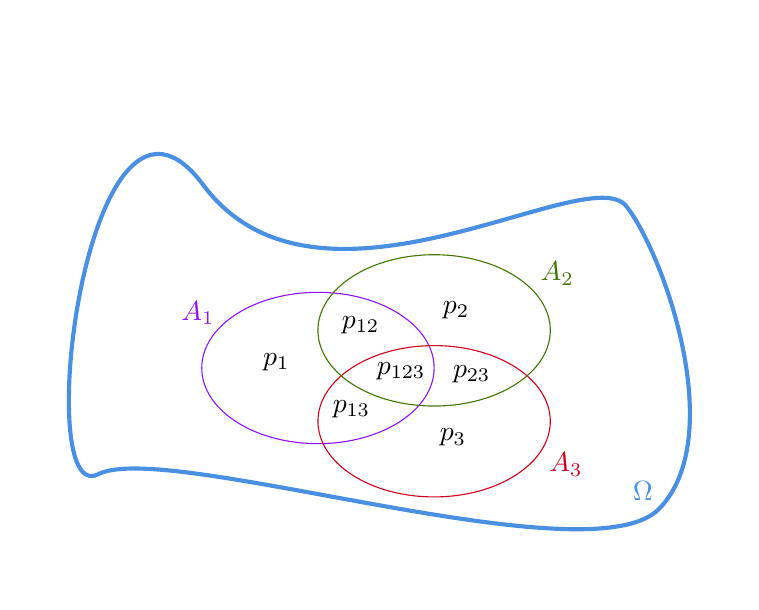
\begin{tikzpicture}[x=0.55pt,y=0.55pt,yscale=-1,xscale=1]
		%uncomment if require: \path (0,300); %set diagram left start at 0, and has height of 300
		
		%Shape: Ellipse [id:dp6153307684562654] 
		\draw  [color={rgb, 255:red, 144; green, 19; blue, 254 }  ,draw opacity=1 ] (240.33,149.72) .. controls (240.33,122.26) and (274.51,100) .. (316.67,100) .. controls (358.82,100) and (393,122.26) .. (393,149.72) .. controls (393,177.17) and (358.82,199.43) .. (316.67,199.43) .. controls (274.51,199.43) and (240.33,177.17) .. (240.33,149.72) -- cycle ;
		%Shape: Ellipse [id:dp9407450341012902] 
		\draw  [color={rgb, 255:red, 208; green, 2; blue, 27 }  ,draw opacity=1 ] (316.67,184.72) .. controls (316.67,157.26) and (350.84,135) .. (393,135) .. controls (435.16,135) and (469.33,157.26) .. (469.33,184.72) .. controls (469.33,212.17) and (435.16,234.43) .. (393,234.43) .. controls (350.84,234.43) and (316.67,212.17) .. (316.67,184.72) -- cycle ;
		%Shape: Ellipse [id:dp3952986651350334] 
		\draw  [color={rgb, 255:red, 65; green, 117; blue, 5 }  ,draw opacity=1 ] (316.67,125.02) .. controls (316.67,97.56) and (350.84,75.3) .. (393,75.3) .. controls (435.16,75.3) and (469.33,97.56) .. (469.33,125.02) .. controls (469.33,152.47) and (435.16,174.73) .. (393,174.73) .. controls (350.84,174.73) and (316.67,152.47) .. (316.67,125.02) -- cycle ;
		%Shape: Polygon Curved [id:ds25964226952294633] 
		\draw  [color={rgb, 255:red, 74; green, 144; blue, 226 }  ,draw opacity=1 ][line width=1.5]  (241.33,29.5) .. controls (317.33,131.5) and (494.33,11.5) .. (519.33,43.5) .. controls (544.33,75.5) and (586.33,195.5) .. (540.8,242.27) .. controls (495.27,289.04) and (217.33,196.5) .. (172.33,219.5) .. controls (127.33,242.5) and (165.33,-72.5) .. (241.33,29.5) -- cycle ;
		
		% Text Node
		\draw (521.8,222.67) node [anchor=north west][inner sep=0.75pt]  [color={rgb, 255:red, 74; green, 144; blue, 226 }  ,opacity=1 ]  {$\Omega $};
		% Text Node
		\draw (225.28,104.4) node [anchor=north west][inner sep=0.75pt]  [color={rgb, 255:red, 144; green, 19; blue, 254 }  ,opacity=1 ]  {$A_{1}$};
		% Text Node
		\draw (461.28,78.4) node [anchor=north west][inner sep=0.75pt]  [color={rgb, 255:red, 65; green, 117; blue, 5 }  ,opacity=1 ]  {$A_{2}$};
		% Text Node
		\draw (467,203.83) node [anchor=north west][inner sep=0.75pt]  [color={rgb, 255:red, 208; green, 2; blue, 27 }  ,opacity=1 ]  {$A_{3}$};
		% Text Node
		\draw (279,138.4) node [anchor=north west][inner sep=0.75pt]    {$p_{1}$};
		% Text Node
		\draw (397,104.4) node [anchor=north west][inner sep=0.75pt]    {$p_{2}$};
		% Text Node
		\draw (395,188.12) node [anchor=north west][inner sep=0.75pt]    {$p_{3}$};
		% Text Node
		\draw (330.69,114.4) node [anchor=north west][inner sep=0.75pt]    {$p_{12}$};
		% Text Node
		\draw (324.69,169.4) node [anchor=north west][inner sep=0.75pt]    {$p_{13}$};
		% Text Node
		\draw (403.69,146.4) node [anchor=north west][inner sep=0.75pt]    {$p_{23}$};
		% Text Node
		\draw (353.69,144.4) node [anchor=north west][inner sep=0.75pt]    {$p_{123}$};
		
		
		\end{tikzpicture}
		\caption{}
	\end{figure}\ \\
	Let
	\begin{align*}
	p_1=P(A_1\cap A_2^c\cap A_3^c),\quad p_2=P(A_1^c\cap A_2\cap A_3^c),\quad p_3=P(A_1^c\cap A_2^c\cap A_3), \\
	p_{12}=P(A_1\cap A_2\cap A_3^c),\quad p_{13}=P(A_1\cap A_2^c\cap A_3),\quad p_{23}=P(A_1^c\cap A_2\cap A_3),
	\end{align*} and $p_{123}=P(A_1\cap A_2\cap A_3)$. Then \begin{align*}
	&P(A_1)+P(A_2)+P(A_3)-P(A_1\cap A_2)-P(A_1\cap A_3)-P(A_2\cap A_3)+P(A_1\cap A_2\cap A_3)\\
	&=(p_1+p_{12}+p_{13}+p_{123})+(p_2+p_{12}+p_{23}+p_{123})+(p_3+p_{13}+p_{23}+p_{123})\\
	&-(p_{12}+p_{123})-(p_{13}+p_{123})-(p_{23}+p_{123})+p_{123}\\
	&=p_1+p_2+p_3+p_{12}+p_{13}+p_{23}+p_{123}=P(A_1\cup A_2\cup A_3).
	\end{align*}
\end{proof}
\end{enumerate}
\
\begin{example}
	Pick an integer in $[1,1000]$ at random. Compute the probability that it is divisible neither by 12 nor by 15.
	\begin{proof}[\sol]
		The sample space $S$ consists of the $1000$ integers between $1$ and $1000$, so $\abs{S}=1000$. Let $A_r$ be the subset consisting of integers divisible by $r$. The cardinality of $A_r$ is $\dispsty\floor*{\frac{1000}{r}}$. Note that  $A_r\cap A_s=A_{\lcm(r,s)}$. Thus, \begin{align*}
		1-P(A_{12}\cap A_{15})&=1-P(A_{12})-P(A_{15})+P(A_{12}\cap A_{15})\\
		&=1-P(A_{12})-P(A_{15})+P(A_{60})\\
		&=1-\frac{83}{1000}-\frac{66}{1000}+\frac{16}{1000}=0.867.
		\end{align*}
	\end{proof}
\end{example}
\
\begin{example}
	Sit $3$ men and $4$ women at random in a row. What is the probability that either all the men or all women end up sitting together?
	\begin{proof}[\sol]
		Let $A_1=\set{\text{all women sit together}}$, $A_2=\set{\text{all men sit together}}$,\\ $A_1\cap A_2=\set{\text{both women and men sit together}}$, and so the answer is \[
		P(A_1\cup A_2)=P(A_1)+P(A_2)-P(A_1\cap A_2)=\frac{4!4!}{7!}+\frac{5!3!}{7!}-\frac{2!3!4!}{7!}.
		\]
	\end{proof}
\end{example}
\
\begin{example}
	A group of $3$ Norwegians, $4$ Swedes, and $5$ Finns is seated at random around a table. Compute the probability that at least one of the three groups end up sitting together.
	\begin{proof}[\sol]
		Define $A_N=\set{\text{Norwegians sit together}}$ and similarly $A_S, A_F$. Then we have \begin{align*}
		&P(A_N)=\frac{3!9!}{11!},\quad P(A_N)=\frac{4!8!}{11!},\quad
		P(A_N)=\frac{5!7!}{11!}\\
		&P(A_N\cap A_S)=\frac{3!4!6!}{11!},\quad
		P(A_N\cap A_F)=\frac{3!5!5!}{11!},\quad
		P(A_S\cap A_F)=\frac{4!5!4!}{11!}\\
		&P(A_N\cap A_S\cap A_F)=\frac{3!4!5!2!}{11!}.
		\end{align*} Therefore \[
		P(A_N\cup A_S\cup A_F)=\frac{3!9!+4!8!+5!7!-3!4!6!-3!5!5!-4!5!4!+3!4!5!2!}{11!}.
		\]
	\end{proof}
\end{example}
\
\begin{example}[\textit{Matching Problem}]
	A large company with $n$ employees has a scheme according to which each employee buys a Christmas gift and the gifts are then distributed at random to the employees. What is the probability that someone gets his or her own gift?
	\begin{proof}[\sol]
		Note that this is different from asking, assuming that you are one of the employees, for the probability that \textit{you} get your own gift, which is $1/n$.\\
		\\
		Let $A_i=\set{i\text{-th employee gets his or her own gift}}$. Then, what we are looking for is \[
		P\left(\bigcup_{i=1}^nA_i\right).
		\] Note that \begin{align*}
		&P(A_i)=\frac{1}{n}\ \text{(for all $i$)},\\
		&P(A_i\cap A_j)=\frac{(n-2)!}{n!}=\frac{1}{n(n-1)}\ \text{(for all $i<j$)},\\
		&P(A_i\cap A_j\cap A_k)=\frac{(n-3)!}{n!}=\frac{1}{n(n-1)(n-2)}\ \text{(for all $i<j<k$)},\\
		&P(A_1\cap\cdots\cap A_n)=\frac{1}{n!}.
		\end{align*} Recall that \begin{align*}
		P(A_1\cup\cdots\cup A_n)&=\sum_{i=1}^nP(A_i)\\
		&-\sum_{1\leq i<j\leq n}P(A_i\cap A_j)\\
		&+\sum_{1\leq i<j<k\leq n}P(A_i\cap A_j\cap A_k)\\
		&+\cdots+(-1)^{n-1}P(A_1\cap\cdots\cap A_n)
		\end{align*} and that \begin{align*}
		\exp(x)&=\sum_{k=0}^\infty\frac{x^k}{k!}=1+x+\frac{x^2}{3!}+\frac{x^4}{4!}+\cdots,\\
		\exp(x)&=\lim\limits_{n\to\infty}\left(1+\frac{x}{n}\right)^n.
		\end{align*}Therefore, our answer is \begin{align*}
		n\cdot\frac{1}{n}-\binom{n}{2}\cdot\frac{1}{n(n-1)}+\binom{n}{3}\cdot\frac{1}{n(n-1)(n-2)}-\cdots+(-1)^{n-1}\frac{1}{n!}&=1-\frac{1}{2!}+\frac{1}{3!}+(-1)^{n-1}\frac{1}{n!}\\
		&=1-\frac{1}{e}\approx 0.6321\ \text{(as $n\to\infty$)},
		\end{align*}
	\end{proof}
\end{example}
\
\begin{example}[\it Birthday Problem.]
	Assume that there are $k$ people in the room. What is the probability that there are two who share a birthday? We will ignore leap years, assume all birthdays are equally likely, and generalize the problem a little: from $n$ possible birthdays, sample $k$ times with replacement. \[
	P(\text{a shared birthday})=1-P(\text{no shared birthdays})=1-\frac{n(n-1)\cdots(n-k+1)}{n^k}.
	\] When $n=365$, the lowest $k$ for which the above exceeds $0.5$ is, famously, $k=23$. Some values are given in the following table: \begin{table}[h!]
		\centering\begin{tabular}{c|c}
			$k$ & prob. for $n=365$ \\
			\hline
			$10$ & $0.1169$ \\
			$23$ & $0.5073$ \\
			$41$ & $0.9032$ \\
			$57$ & $0.9901$ \\
			$70$ & $0.9992$ \\
		\end{tabular}
	\end{table}
\end{example}
\
\begin{example}[\it Coupon Collector Problem]
	Within the context of the previous problem, assume that $k\geq n$ and compute $P(\text{all}\ n\ \text{birthdays are represented})$.\begin{proof}[\sol]
		This is described in terms of cereal boxes, each of which contains one of $n$ different cards (coupons), chosen at random. If you buy $k$ boxes, what is the probability that you have a complete collection?\\
		\\
		When $k=n$, our probability is $n!/n^n$. More generally, let \[
		A_i=\set{\text{$i$-th birthday is missing}}.
		\] Then, we need to compute \[
		1-P\left(\bigcup_{i=1}^nA_i\right).
		\] Now, \begin{align*}
		&P(A_i)=\frac{(n-1)^k}{n^k}\ \text{(for all $i$)},\\
		&P(A_i\cap A_j)=\frac{(n-2)^k}{n^k}\ \text{for all $i<j$}, \\
		&P(A_1\cap\cdots\cap A_n)=0
		\end{align*} and our answer is \begin{align*}
		1-P\left(\bigcup_{i=1}^nA_i\right)&=1-n\left(\frac{n-1}{n}\right)^k+\binom{n}{2}\left(\frac{n-2}{n}\right)^k-\cdots+(-1)^{n-1}\binom{n}{n-1}\left(\frac{1}{n}\right)^k \\
		&=\sum_{i=0}^n\binom{n}{i}(-1)^i\left(1-\frac{i}{n}\right)^k.
		\end{align*}
	\end{proof}
\end{example}
\
\begin{example}
	Roll a die $12$ times. Compute the probability that a number occurs $6$ times and two other numbers occur three times each.\begin{proof}[\sol]
		The number of outcomes is $6^12$. To count the number of good outcomes: \begin{enumerate}
			\item Pick the number that occurs $6$ times: $\binom{6}{1}=6$ choices.
			\item Pick the two numbers that occurs $3$ times each: $\binom{5}{2}$ choices.
			\item Pick slots (rolls) for the number that occurs $6$ times: $\binom{12}{6}$ choices.
			\item Pick slots (rolls) for one of the numbers that occurs $3$ times: $\binom{6}{3}$ choices.
		\end{enumerate} Therefore, out probability is $\dispsty\frac{6\binom{5}{2}\binom{12}{6}\binom{6}{3}}{6^12}$.
	\end{proof}
\end{example}

\subsection{Problems}

\newpage
\section{Conditional Probability and Independence}
\subsection{Introduction}
\begin{example}
	Assume that you have a big with $11$ cubes, $7$ of which have a fuzzy surface and $4$ are sooth. Out of the $7$ fuzzy ones, $3$ are red and $4$ are blue; out of $4$ smooth ones, $2$ are red and $2$ are blue. So, there are $5$ red and $6$ blue cubes. Other than color and fuzziness, the cubes have no other distinguishing characteristic.\\
	\\
	Your experiment clearly has $11$ outcomes. Consider the events $R, B, F, S$ that selected cube is red, blue, fuzzy, and smooth, respectively. We observed $P(R)=5/11$. FOr the probability of a red cube, \textit{conditioned on it being fuzzy}, we do not have notation, so we introduce it here: $P(R|F)=3/7$. Note that this also equals \[
	\frac{P(R\cap F)}{P(F)}=\frac{3/11}{7/11}=\frac{3}{7}.
	\]
\end{example}
\
\begin{example}
	Here is a question asked on \textit{Wall Street job interviews}.\begin{quote}
		``Let's play a game of Russian roulette. You are tied to your chair. Here's a gun, a revolver. Here's the barrel of the gun, six chambers, all empty. Now watch me as I put \textit{two} bullets into the barrel, into \textit{two adjacent chambers}. I close the barrel and spin it. I put a gun to your head and pull the trigger. Click. Lucky you! Now I'm going to pull the trigger one more time. Which would you prefer: that I \textcolor{blue}{\it spin the barrel first} or that I \textcolor{red}{\it just pull the trigger}?''
	\end{quote} Assume that the barrel rotates clockwise after the hammer hits and is pulled back. You are given the choice between an \textcolor{blue}{\it unconditional} and a \textcolor{red}{\it conditional} probability of death. \begin{itemize}
	\item The former, if the barrel is spin again, remains $1/3$.
	\item The latter, if the trigger is pulled without the extra spin, equals the probability that the hammer clicked on an empty slot, which is next to a bullet in the counterclockwise direction, and equals $1/4$.
\end{itemize}
\end{example}

\subsection{Conditional Probabilities}
\begin{tcolorbox}[colback=white]
	\begin{definition}
		Assume that $P(B)>0$. The \textbf{conditional probability of $A$ given $B$} equals \[
		P(A|B)=\frac{P(A\cap B)}{P(B)}.
		\]
	\end{definition}
\end{tcolorbox} For a fixed condition $B$, and acting on events $A$, the conditional probability $Q(A)=P(A|B)$ satisfies the three axioms of probability. Thus, $Q$ is another probability assignment all consequences of the axioms are valid for it.\
\\
\begin{example}
	Toss two fair coins, blindfolded. Somebody tells you that you tossed at least one Heads. What is the probability that both tosses are Heads?\begin{proof}[\sol]
		Here $A=\set{\text{both}\ H}$, $B=\set{\text{at least one}\ H}$, and \[
		P(A|B)=\frac{P(A\cap B)}{P(B)}=\frac{P(\text{both $H$})}{P(\text{at least one $H$})}=\frac{1/4}{3/4}=\frac{1}{3}.
		\]
	\end{proof}
\end{example}\
\\
\textcolor{purple}{\bf Advanced.}\quad If $P(A)=0$, then the event $A$ cannot be occurred. (\textcolor{red}{\bf False})
\begin{proof}
	\ \begin{figure}[h!]
		\centering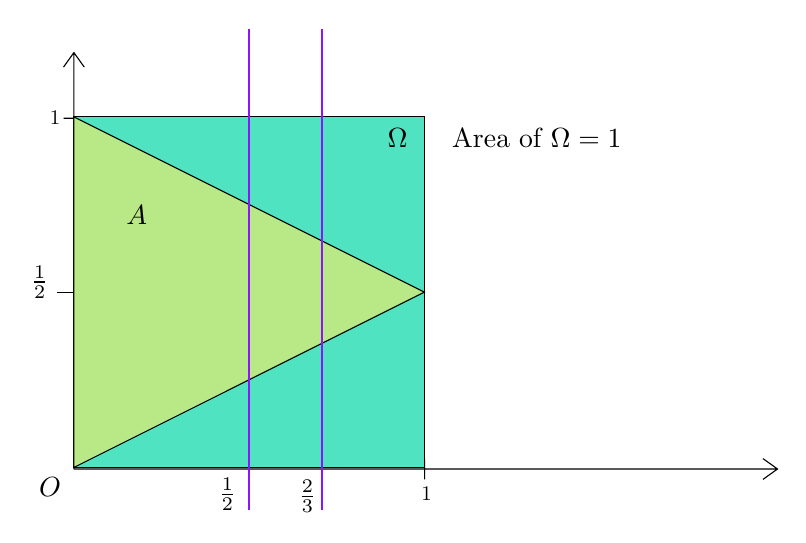
\begin{tikzpicture}[x=0.75pt,y=0.75pt,yscale=-1,xscale=1]
		%uncomment if require: \path (0,300); %set diagram left start at 0, and has height of 300
		
		%Shape: Axis 2D [id:dp5017244711300923] 
		\draw  (181,237.43) -- (520,237.43)(181,36.8) -- (181,237.43) -- cycle (513,232.43) -- (520,237.43) -- (513,242.43) (176,43.8) -- (181,36.8) -- (186,43.8) (350,232.43) -- (350,242.43)(176,68.43) -- (186,68.43) ;
		\draw   (357,249.43) node[anchor=east, scale=0.75]{1} (178,68.43) node[anchor=east, scale=0.75]{1} ;
		%Shape: Square [id:dp23140297522236564] 
		\draw  [fill={rgb, 255:red, 80; green, 227; blue, 194 }  ,fill opacity=1 ] (181,67.8) -- (349.87,67.8) -- (349.87,236.67) -- (181,236.67) -- cycle ;
		%Straight Lines [id:da2257499784737702] 
		\draw    (172.8,152.23) -- (190.8,152.23) ;
		%Shape: Triangle [id:dp5047032781530383] 
		\draw  [fill={rgb, 255:red, 184; green, 233; blue, 134 }  ,fill opacity=1 ] (349.87,152.23) -- (181,236.67) -- (181,67.8) -- cycle ;
		%Straight Lines [id:da2685047581044211] 
		\draw [color={rgb, 255:red, 144; green, 19; blue, 254 }  ,draw opacity=1 ][line width=0.75]    (265.43,25.3) -- (265.43,257.3) ;
		%Straight Lines [id:da038736665622387756] 
		\draw [color={rgb, 255:red, 144; green, 19; blue, 254 }  ,draw opacity=1 ][line width=0.75]    (300.43,25.3) -- (300.43,257.3) ;
		
		% Text Node
		\draw (163,240.4) node [anchor=north west][inner sep=0.75pt]    {$O$};
		% Text Node
		\draw (330.87,72.2) node [anchor=north west][inner sep=0.75pt]    {$\Omega $};
		% Text Node
		\draw (362,71.8) node [anchor=north west][inner sep=0.75pt]   [align=left] {Area of $\displaystyle \Omega =1$};
		% Text Node
		\draw (159,138.13) node [anchor=north west][inner sep=0.75pt]    {$\frac{1}{2}$};
		% Text Node
		\draw (205,109.4) node [anchor=north west][inner sep=0.75pt]    {$A$};
		% Text Node
		\draw (249.43,240.4) node [anchor=north west][inner sep=0.75pt]    {$\frac{1}{2}$};
		% Text Node
		\draw (287.93,241.4) node [anchor=north west][inner sep=0.75pt]    {$\frac{2}{3}$};
		
		
		\end{tikzpicture}
		\caption{}
	\end{figure}\ \\ 
	From Fig 4., \[
	P(A)=P[(x,y)\in A]=\frac{1}{2}
	\] and \[
	P(\set{x=1/2})=P(\set{x=2/3})=0.
	\] Then \begin{align*}
	P\left(A|\set{x=1/2}\right)=\frac{1}{2},\\
	P\left(A|\set{x=2/3}\right)=\frac{1}{3}.
	\end{align*}
\end{proof}
\
\begin{example}
	Toss a coin $10$ times. If you know (a) that exactly $7$ Heads are tossed, (b) that at least $7$ Heads are tossed, what is the probability that your first toss is Heads?\begin{proof}[\sol]
		For (a), \[
		P(\text{first toss $H$}|\text{exactly $7$ H's})=\frac{\binom{9}{6}\cdot\frac{1}{2^{10}}}{\binom{10}{7}\cdot\frac{1}{2^{10}}}=\frac{7}{10}=0.7.
		\] If you choose $7$ tosses out of $10$ at random, the first toss is included in your choice with probability $7/10$.\\
		\\
		For (b), the answer is, after canceling $1/2^{10}$, \[
		\frac{\binom{9}{6}+\binom{9}{7}+\binom{9}{8}+\binom{9}{9}}{\binom{10}{7}+\binom{10}{8}+\binom{10}{9}+\binom{10}{10}}=\frac{65}{88}\approx 0.7388.
		\]\\
		\\ Clearly, the answer should be a little larger than before, because this condition is more advantageous for Heads.
	\end{proof}
\end{example}

\subsection{Bayes' Formula}
\begin{tcolorbox}[colback=white]
	Conditional probabilities are sometimes \textit{given}, or can be easily determined, especially in sequential random experiments. Then, we can use \begin{align*}
	&P(A_1\cap A_2)=P(A_1)P(A_2|A_1),\\
	&P(A_1\cap A_2\cap A_3)=P(A_1)P(A_2|A_1)P(A_3|A_1\cap A_2),
	\end{align*} etc.
\end{tcolorbox}
\
\begin{example}
	An urn contains $10$ black and $10$ white balls. Draw $3$ (a) without replacement, and (b) with replacement. What is the probability that all three are white?\begin{proof}[\sol]
		Part (a):\begin{enumerate}
			\item Number of outcomes: $\binom{20}{3}$.
			\item Number of ways to select $3$ balls out of $10$ white ones: $\binom{10}{3}$.
		\end{enumerate} Our probability is then $\dispsty\frac{\binom{10}{3}}{\binom{20}{3}}$.\\
	\\
	To do this problem another way, imagine drawing the balls sequentially. Then, we are computing the probability of the intersection of the three events: $P(1\text{st ball is white}, 2\text{nd ball is white}, 3\text{rd ball is white})$. The relevant probabilities are:\begin{enumerate}
		\item $P(1\text{st ball is white})=1/2$.
		\item $P(2\text{st ball is white}|1\text{st ball is white})=9/19$.
		\item $P(1\text{st ball is white}|1\text{st two picked are white})=8/18$.
	\end{enumerate} Our probability is, then, the product $1/2\cdot9/19\cdot8/18$, which equals, as it must, what we obtained before.\\
	\\
	This approach is particularly easy in case (b), where the previous colors of the selected balls do not affect the probabilities at subsequent stages. The answer, therefore, is $(1/2)^3$ by\[
	P(A_1\cap A_2\cap A_3)=P(A_1)P(A_2|A_1)P(A_3|A_1\cap A_2).
	\]
	\end{proof}
\end{example}
\
\begin{tcolorbox}[colback=white]
	\begin{theorem}[\bf First Bayes' Formula]
		Assume that $F_1\cdots, F_n$ are pairwise disjoint and that $\bigcup_{i=1}^nF_i=\Omega$, that is, exactly one of them always happens. In other worlds, $F_i$ is partition of $\Omega$. Then for an event $A$, 
		\begin{align*}
		P(A)&=P(F_1)P(A|F_1)+P(F_2)P(A|F_2)+\cdots P(F_n)P(A|F_n).
		\end{align*} It is also called \textbf{Law of Total Probability}.
	\end{theorem}\tcblower\begin{proof}
	\begin{align*}
	P(A)&=P(A\cap\Omega)\\
	&=P\left[A\cap\left(\bigcup_{i=1}^nF_i\right)\right]\\
	&=P\left[(A\cap F_1)\cup(A\cap F_2)\cup\cdots\cup(A\cap F_n)\right]\\
	&=P(A\cap F_1)+P(A\cap F_2)+\cdots+P(A\cap F_n)\\
	&=P(F_1)P(A|F_1)+P(F_2)P(A|F_2)+\cdots+P(F_n)P(A|F_n).
	\end{align*}
\end{proof}
\end{tcolorbox} We call an instance of using this formula ``computing the probability by conditioning on which of the events $F_i$ happens.'' The formula is useful in sequential experiments, when you face different experimental conditions at the second stage depending on what happens at the first stage. Quite often, there are just two events $F_i$, that is, an event $F$ and its complement $F^c$, and we are thus conditioning on whether $F$ happens or not.\
\\
\begin{example}
	Flip a fair coin. If you toss Heads, roll $1$ die. If you toss Tails, roll $2$ dice. Compute the probability that you roll exactly one $6$.\begin{proof}[\sol]
		Here you condition on the outcome of the coin toss, which could be Head (event $F$) or Tail (event $F^c$). If $A=\set{\text{exactly one}\ 6}$, then $P(A|F)=1/6$, $P(A|F^c)=2\cdot 5/{36}$, $P(F)=P(F^c)=1/2$, and so \[
		P(A)=P(F)P(A|F)+P(F^c)P(A|F^c)=\frac{2}{9}.
		\]
	\end{proof}
\end{example}
\
\begin{example}
	Roll a die, then select at random, without replacement, as many cards from the deck as the number shown on the die. What is the probability that you get at least one Ace?\begin{proof}[\sol]
		Let $F_i=\set{\text{number shown on the die is}\ i}$, for $i=1,\cdots,6$. Clearly, $P(F_i)=1/6$. If $A$ is the event that you get at least one Ace, \begin{enumerate}
			\item $P(A|F_1)=1/13$,
			\item In general, for $i>1$, $P(A|F_i)=1-\binom{48}{i}/\binom{52}{i}$.
		\end{enumerate} Therefore, by 1st Bayes' formula, \[
	P(A)=\frac{1}{6}\left(\frac{1}{13}+1-\frac{\binom{48}{2}}{\binom{52}{2}}+1-\frac{\binom{48}{3}}{\binom{52}{3}}+1-\frac{\binom{48}{4}}{\binom{52}{4}}+1-\frac{\binom{48}{5}}{\binom{52}{5}}+1-\frac{\binom{48}{6}}{\binom{52}{6}}+1\right)
	\]
	\end{proof}
\end{example}
\
\begin{example}[\it Coupon collector problem - revisited] As promised, we will develop a computationally much better formula than the one in Example 3.9. This will be another example of \textit{conditioning}, whereby you (1) \textit{reinterpret} the problem as a sequential experiment and (2) use Bayes' formula with ``conditions'' $F_i$ being relevant events at the first stage of the experiment.\\
\\
Let $P_{k,r}$ be the probability that exactly $r$ (out of a total of $n$) birthdays are represented among $k$ people, we call the even $A$; that is, \[
P(A)=p_{k,r}\quad(r\leq n\leq k).
\] We will fix $n$ and let $k$ and $r$ be variable. Note that $p_{k,r}$ is what we computed by the \textbf{inclusion-exclusion formula}.\\
\\ At the first stage you have $k-1$ people; then the $k$-th person arrives on the scene. Let \begin{align*}
F_1&:\ \text{the events that there are $r$ birthdays represented among the $k-1$ people,}\\
F_2&:\ \text{the events that there are $r-1$ birthdays represented among the $k-1$ people,}\\
F_3&:\ \text{the events that any other number of birthdays represented among the $k-1$ people}.
\end{align*} Clearly, $P(A|F_3)=0$ as the newcomer contributes either \textbf{0} or \textbf{1} new birthdays. Moreover, $P(A|F_1)=r/n$, the probability that the newcomer duplicates one of the existing $r$ birthdays, and $P(A|F_2)=n-r(-1)/n$ the probability that the newcomer does not duplicate any of the existing $r-1$ birthdays.\\
\\
Therefore, \begin{align*}
p_{k,r}=P(A)&=P(A|F_1)P(F_1)+P(A|F_2)P(F_2)\\
&=\frac{r}{n}p_{k-1,r}+\frac{n-r+1}{n}\cdot p_{k-1,r-1}
\end{align*} for $k,r\geq 1$, and this, together with the boundary conditions \begin{align*}
p_{0,0}&=1\\
P_{k,r}&=0,\ \text{for $0\leq k<r$},\\
P_{k,0}&=0,\ \text{for $k>0$},\\
\end{align*} makes the computation fast and precise. In Example 3.9, by using the \textit{inclusion-exclusion formula}, we have obtained that for \[
P(\text{complete collection})=1-P\left(\bigcup_{i=1}^nA_i\right),
\] where $A_i=\set{i\text{-th birthday is missing}}$, \begin{align*}
1-P\left(\bigcup_{i=1}^nA_i\right)&=1-n\left(\frac{n-1}{n}\right)^k+\binom{n}{2}\left(\frac{n-2}{n}\right)^k-\cdots+(-1)^n\binom{n}{n-1}\left(\frac{1}{n}\right)^k\\
&=\sum_{i=0}^{n}\binom{n}{i}(-1)^i\left(1-\frac{i}{n}\right)^k.
\end{align*}
\end{example}
\
\begin{tcolorbox}[colback=white]
	\begin{theorem}[\bf Second Bayes' Formula]
		Let $F_1,\cdots,F_n$ and $A$ be as in \textbf{Theorem 4.1}. Then \[
		P(F_j|A)=\frac{P(F_j\cap A)}{P(A)}=\frac{P(A|F_j)P(F_j)}{P(A_1|F_1)+\cdots+P(A|F_n)P(F_n)}.
		\] An event $F_j$ is often called a \text{\normalfont\bf hypothesis}, $P(F_j)$ its \text{\normalfont\bf prior probability}, and $P(F_j|A)$ its \text{\normalfont\bf posterior probability}.
	\end{theorem}
\end{tcolorbox} Note that \[
\underset{\text{Posterior}}{P(A|B)}=\frac{\overset{\text{Likelihood}}{P(B|A)}\cdot\overset{\text{Prior}}{P(A)}}{\underset{\text{Evidence}}{P(B)}}.
\]

\begin{example}
	We have a fair coin and and unfair coin, which always comes out Heads. Choose one at random, toss it twice. It comes out Head both times. What is the probability that the coin is fair?
	\begin{proof}[\sol]
		The relevant events are $F=\set{\text{fair coin}}$, $U=\set{\text{unfair coin}}$, and $B=\set{\text{both tosses}\ H}$. Then $P(F)=P(U)=1/2$ (as each coin is chosen with equal probability). Moreover, $P(B|F)=1/4$, and $P(B|U)=1$. Our probability then is \[
		P(F|B)=\frac{P(F)P(B|F)}{P(F)P(B|F)+P(U)P(B|U)}=\frac{1/2\cdot 1/4}{1/2\cdot1/4+1/2\cdot1}=\frac{1}{5}.
		\]
	\end{proof}
\end{example}
\
\begin{example}
	A factory has three machines, $M_1, M_2$, and $M_3$, that produce items (say, lightbulbs). It is impossible to tell which machine produced a particular item, but some are defective. Here are the known numbers: \begin{table}[h!]
		\centering
		\begin{tabular}{|c|c|c|}
			\toprule
			machine & proportion of item made & prob. any made item is defective\\
			\hline
			$M_1$ & $0.2$ & $0.001$\\
			\hline
			$M_2$ & $0.3$ & $0.002$\\
			\hline
			$M_3$ & $0.5$ & $0.003$\\
			\bottomrule
		\end{tabular}
	\end{table}\\ You pick an item, test is, and find it is defective. What is the probability that it was made by machine $M_2$?
	\begin{proof}[\sol]
		The best way to think about this random experiment is as a two-stage procedure. First you choose a machine with the probabilities given by the proportion. Then, that machine produces an item, which you then proceed to test. (Indeed, this is the same as choosing the item from a large number of them and testing it.)\\
		\\
		Let $D$ be the event that an item is defective and let $M_i$ also denote the event that the item was made by machine $i$. Then, $P(D|M_1)=0.001$, $P(D|M_2)=0.002$, $P(D|M_3)=0.003$, $P(M_1)=0.2$, $P(M_2)=0.3$, $P(M_3)=0.5$, and so \[
		P(M_2|D)=\frac{0.002\cdot 0.3}{0.001\cdot0.2+0.002\cdot0.3+0.003\cdot0.5}\approx 0.26.
		\]
	\end{proof}
\end{example}
\
\begin{example}
	Assume 10\% of people have a certain disease. A test gives the correct diagnosis with probability of 0.8; that is, if the person is sick, the test will be positive with probability 0.8, but if the person is not sick, the test will be positive with probability 0.2. A \textit{random person} from the population has tested positive for the disease. What is the probability that he is actually sick? (No, it is not 0.8.) \begin{proof}[\sol]
		Let us define the three relevant events: $S=\set{\text{sick}}$, $H=\set{\text{healthy}}$, $T=\set{\text{tested positive}}$. Now, $P(H)=0.9, P(S)=0.1, P(T|H)=0.2$, and $P(T|S)=0.8$. We are interested in $S^c=H$. Thus, \[
		P(S|T)=\frac{P(T|S)P(S)}{P(T|S)P(S)+P(T|H)P(H)}=\frac{8}{26}\approx0.31.
		\]
	\end{proof}
\end{example}
\
\begin{example}[\it O. J. Simpson's first trial,\ \normalfont 1995]
	The famous sports star and media personality O. J. Simpson wa on trial in Los Angeles for murder of his wife and her boyfriend. One of the may issues was whether Simpson's history of spousal abuse could be presented by prosecution at the trial; that is, whether this history was ``probative,'' \ie, it had some evidentiary value, or whether it was merely ``prejudicial'' and should be excluded. Alan Dershowitz, a famous professor of law at Harvard and a consultant for the defense, was claiming the latter, citing the statistics that $<0.1\%$ of men who abuse their wives and up killing them. As J. F. Merz and J. C. Caulkins pointed out in the journal \textit{Chance} (Vol. 8. 1995, pg. 14), this was th wrong probability to look at!\\
	\\
	Dershowitz states that ``a considerable number'' of wife murderers had previously assaulted them, although ``some'' did not. So, we will (conservatively) say that $P(A|M)=0.5$. (The two-stage experiment then is: choose a murdered woman at random; at the first stage, she is murdered by her partner, or not, with stated probabilities; at the second stage, she is among the abused women, or not, with probabilities depending on the outcome of the first stage.) By Bayes' formula, \[
	P(M|A)=\frac{P(M)P(A|M)}{P(M)P(A|M)+P(M^c)P(A|M^c)}=\frac{(0.29)(0.5)}{(0.29)(0.5)+(0.71)(0.05)}=\frac{29}{36.1}\approx0.8.
	\] The law literature studiously avoids quantifying concepts such as probative value and reasonable doubt. Nevertheless, we can probably say that 80\% is considerably too high compared to the prior probability of 29\%, to use as a \textit{sole} argument that the evidence is not probative.
\end{example}

\subsection{Independent Events}
\begin{tcolorbox}[colback=white]
	\begin{definition}[\bf Independence]
		Events $A$ and $B$ are \textbf{independent} if $P(A\cap B)=P(A)P(B)$ and \textbf{dependent} (or \textbf{correlated}) other wise.
	\end{definition}
\end{tcolorbox} Assume that $P(B)>0$, one could rewrite the condition for independence, \[
P(A|B)=P(A),
\] so the probability of $A$ is unaffected by knowledge that $B$ occurred. Also, if $A$ and $B$ are independent.
\\
\begin{note}
	We claim that $A$ and $B$ are independent if and only if $A$ and $B^c$ are independent. \[
	P(A\cap B^c)=P(A)-P(A\cap B)=P(A)-P(A)P(B)=P(A)(1-P(B))=P(A)P(B^c),
	\] so $A$ and $B^c$ are also independent.
\end{note}
\
\begin{example}
	Pick a random card from a full deck. Let $A=\set{\text{card is an Ace}}$ and $R=\set{\text{card is red}}$. Are $A$ and $R$ independent?\begin{proof}[\sol]
		We have $P(A)=1/13$, $P(R)=1/2$, and, as there are two red Aces, $P(A\cap R)=2/52=1/26$. The two events are independent---the proportion of aces among red card is the same as the proportion among all cards. That is, $P(A\cap R)=P(A)P(R)$.\\
		\\
		Now, pick two cards out of the deck sequentially without replacement. Are $F=\set{\text{first card in an Ace}}$ and $S=\set{\text{second card is an Ace}}$ independent? Now $P(F)=P(S)=1/13$ and $P(S|F)=3/51$, so they are not independent. Note that \[
		P(S)=P(F)P(S|F)+P(F^c)P(S|F^c).
		\]
	\end{proof}
\end{example}
\
\begin{example}
	Toss 2 fair coins and let $F=\set{\text{Heads on 1st toss}}$, $S=\set{Heads on 2nd toss}$. These are independent. You will notice that here the independence is in fact and assumption.\\
	\\
	How do we define independence of more than two events? We say that events $A_1,A_2,\cdots, A_n$ are \textit{independent} if \[
	P(A_{i1}\cap\cdots\cap A_{ik})=P(A_{i_1})P(A_{i_2})P(A_{i_k}),
	\] where $1\leq i_1<i_2<\cdots<i_k\leq n$ are arbitrary indices. The occurrence of any combination of events does not influence the probability of others. Again, it can be shown that, in such a collection of independent events, we can replace an $A_i$ by $A_i^c$ and the events remain independent.
\end{example}
\
\begin{example}
	Roll a four sided fair die, that is, choose one of the numbers 1, 2, 3, 4 at random. Let $A=\set{1,2}$, $B=\set{1,3}$, $C=\set{1,4}$. Check that these are pairwise independent (each pair is independent), but not independent.\begin{proof}[\sol]
		Indeed, $P(A)=P(B)=P(C)=1/2$ and $P(A\cap B)=P(A\cap C)=P(B\cap C)=1/4$ and pairwise independence follows. However, \[
		P(A\cap B\cap C)=\frac{1}{4}\neq\frac{1}{8}.
		\] The simple reason for lack of independence is $(A\cap B)\subset C$.
	\end{proof}
\end{example}
\
\begin{example}
	You roll a die, your friend tosses a coin. \begin{itemize}
		\item If you roll 6, you win outright.
		\item If you do not roll 6 and your friend tossed Heads, you lose outright.
		\item If neither, the game is repeated until decided.
	\end{itemize} What is the probability that you win?\begin{proof}[\sol]
	One way to solve this problem certainly is this: \begin{align*}
	P[\text{win}]&=P[\text{win on 1st round}]+P[\text{win on 2nd round}] + P[\text{win on 3rd round}]+\cdots\\
	&=\frac{1}{6}+\left(\frac{5}{6}\cdot\frac{1}{2}\right)\frac{1}{6}+\left(\frac{5}{6}\cdot\frac{1}{2}\right)^2\frac{1}{6}+\cdots\\
	&=\frac{1}{6}\left[1+\left(\frac{5}{12}\right)+\left(\frac{5}{12}\right)^2+\cdots\right]=\frac{1}{6}\left(\frac{1}{1-5/12}\right)=\frac{2}{7}.
	\end{align*} \textit{Important note: we have implicitly assumed independence between the coin and the die, as well as between different tosses and rolls. This is very common in problems such as this!}\\
	\\
	You can avoid the nuisance, however, by the following trick. Let \begin{align*}
	D&=\set{\text{game is decided on 1st round}},\\
	W&=\set{\text{you win}}.
	\end{align*} The events $D$ and $W$ are independent, which one can certainly check by computation, but, in fact, there is a very good reason to conclude so immediately. The crucial observation is that, provided that the game is not decided in the 1st round, you are thereafter facing the same game with the smae winning probability; thus \[
	P(W|D^c)=P(W).
	\] In other words, $D^c$ and $W$ are independent and then so are $D$ and $W$. and therefore \[
	P(W)=P(W|D).
	\] This means that one can solve this problem by computing the relevant probabilities for the 1t round: \[
	P(W)=P(W|D)=\frac{P(W\cap D)}{P(D)}=\frac{1/6}{1/6+5/6+1/2}=\frac{2}{7},
	\] which is our answer.
\end{proof}
\end{example}
\
\begin{example}[\it Craps]
	Many casinos allow you to bet even money on the following game. Two dice are rolled an the sum $S$ is observed. \begin{itemize}
		\item If $S\in\set{7,11}$, you win immediately.
		\item If $S\in\set{2,3,12}$, you lose immediately.
		\item If $S\in\set{4,5,6,8,9,10}$, the pair of dice is rolled repeatedly until one of the following happens: \begin{itemize}
			\item $S$ repeats, in which case you win.
			\item $7$ appears, in which case you lose.
		\end{itemize}
	\end{itemize} What is the winning probability?\begin{proof}[\sol]
	Let us look at all possible ways to win: \begin{enumerate}
		\item For $P(W)=P(F)+P(D)$, where $W$ is event of winning, $F$ is win on $1^{\text{st}}$, and $D$ is win on after $2^{\text{nd}}$, we have $P(F)=8/36$.
		\item Otherwise, $P(D)=P(D_4)+P(D_5)+\cdots+P(D_10)$, where $D_i$ is a event of ``$1^{\text{st}}$ roll $= i\ \text{and win}$''.
	\end{enumerate} Using Bayes' formula $P(D_i)=P(\set{1^{\text{st}}\ \text{roll}}\cap\set{\text{win}})=P(\text{roll}\ i|\text{roll}\ i\ \text{or}\ 7)$, \[
	P(\text{win})=\frac{8}{36}+2\left(\frac{3}{36}\cdot\frac{1}{3}+\frac{4}{36}\cdot\frac{2}{5}+\frac{5}{36}\cdot\frac{5}{11}\right)\approx0.4929,
	\] a decent game by casino standards.
	\end{proof}
\end{example}

\subsection{Bernoulli trials}
\begin{tcolorbox}[colback=white]
	Assume $n$ independent experiments, each of which is a success with probability $p$ and, thus, failure with probability $1-p$. In sequence of $n$ \textbf{Bernoulli trials}, \[
	P[\text{exactly $k$ successes}]=\binom{n}{k}p^k(1-p)^{n-k}.
	\]
\end{tcolorbox} This is because the successes can occur on any subset $S$ of $k$ trials out of $n$, \ie, on any $S\subset\set{1,\cdots,n}$ with cardinality $k$. These possibilities are disjoint, as exactly $k$ successes cannot occur on two different such sets. There are $\binom{n}{k}$ such subsets; if we fix such an $S$, then successes must occur on $k$ trials in $S$ and failures on all $n-k$ trials not in $S$; the probability that this happens, by the assumed independence, is $p^k(1-p)^{n-k}$.
\\
\begin{example}
	A machine produces items which are independently defective with probability $p$. Let us compute a few probabilities: \begin{enumerate}
		\item $P[\text{exactly two items among the first 6 are defective}]=\dispsty\binom{6}{2}p^2(1-p)^2$.
		\item $P[\text{exactly one items among the first 6 is defective}]=1-P[\text{no defects}]=1-(1-p)^6$.
		\item $P[\text{at least 2 items among the first 6 are defective}]=1-(1-p)^6-6p(1-p)^5$.
		\item $P[\text{exactly 100 items are made before 6 defective are found}]$ equals\\ $P[\text{100th item defective, exactly 5 items among 1st 99 defective}]$$=\dispsty p\binom{99}{5}p^5(1-p)^{94}$.
	\end{enumerate}
\end{example}
\
\begin{example}[\it Problem of Points]
	This involves finding the probability of $n$ successes before $m$ failures in a sequence of Bernoulli trials. Let us call this probability $p_{n,m}$.\begin{align*}
	p_{n,m}&=P[\text{in the first $m+n-1$ trials, the number of successes is $\geq n$}]\\
	&=\sum_{k=n}^{n+m-1}\binom{n+m-1}{k}p^k(1-p)^{n+m-1-k}.
	\end{align*} The problem is solved, but it needs to be pointed out that computationally this is not the best formula. It is much more efficient to use the recursive formula obtained by conditioning on the outcome of the first trial. Assume that $m,n\geq 1$. Then, \begin{align*}
	p_{n,m}&=P[\text{first trial is a success}]\cdot P[\text{$n-1$ successes before $m$ failures}]\\
	&=P[\text{first trial is a success}]\cdot P[\text{$n$ successes before $m-1$ failures}]\\
	&=p\cdot p_{n-1,m}+(1-p)\cdot p_{n,m-1}.
	\end{align*} Together with boundary conditions, valid for $m,n\geq 1$, \[
	p_{n,0}=0,\quad p_{0,m}=1,
	\] which allows for very speedy and precise computations for large $m$ and $n$.
\end{example}
\
\begin{example}[\it Best of 7]
	Assume that two equally matched teams, $A$ and $B$, play a series of games and that the first team that wins four games is the overall winner of the series. As it happens, team $A$ lost the first game. What is the probability it will win the series? Assume that the games are Bernoulli trials with success probability $1/2$. We have \begin{align*}
	P[\text{$A$ wins the series}]&=P[\text{4 sucesses before 3 failures}]\\
	&=p_{n,m}(n=4, m=3)\\
	&=\sum_{k=4}^{6}\binom{6}{k}\left(\frac{1}{2}\right)^6=\frac{15+6+1}{2^6}\approx0.3438.
	\end{align*}
\end{example}
\
\begin{example}[\bf Branch Matchbox Problem]
	A mathematician carries two matchboxes, each originally containing $n$ matches. Each time he needs a match, he is equally likely to take it from either box. What is the probability that, upon reaching for a box and finding it empty, there are exactly $k$ matches still in the other box? Here, $0\leq k\leq n$.\\
	\\
	Let $A_1$ be the event that matchbox 1 is the one discovered empty and that, at that instant, matchbox 2 contains $k$ matches. Before this point, he has used $n+n-k$ matches, $n$ from matchbox $1$ and $n-k$ from matchbox 2. This means that he has reached for box 1 exactly $n$ times in $(n+n-k)$ trials and for the last time at the $(n+1+n-k)$-th trial. Therefore, our probability is \[
	2P(A_1)=2\cdot\frac{1}{2}\binom{2n-k}{n}\frac{1}{2^{2n-k}}=\binom{2n-k}{n}\frac{1}{2^{2n-k}}.
	\]
\end{example}
\
\begin{example}
	Each day, you independently decide, with probability $p$, to flip a fair coin. Otherwise, you do noting. (a) What is the probability of getting exactly 10 Heads in the first 20 days? (b) What is the probability of getting 10 Heads before 5 Tails?\\
	\\
	For (a), the probability of getting Heads is $p/2$ independently each day, so the answer is \[
	\binom{20}{10}\left(\frac{p}{2}\right)^{10}\left(1-\frac{p}{2}\right)^10.
	\] For (b), you can disregard days at which you do not flip, to get \[
	\sum_{k=10}^{14}\binom{14}{k}\frac{1}{2^{14}}=p_{n,m}(n=10, m=5).
	\]
\end{example}
\
\begin{example}
	You roll a die and your score is the number shown on the die. Your friend rolls five dice and his score is the number of 6' shown. Compute (a) the probability of event $A$ that the two scores are equal and (b) the probability of event $B$ that your friend's score is strictly lager than yours.\begin{proof}[\sol]
		In both cases we will condition on your friend's score---this works a little better in case (b) than conditioning on your score. Let $F_i (i=0,\cdots,5)$ be the event that your friend's score is $i$. Then, $P(A|F_i)=\frac{1}{6}$ if $i\geq 1$ and $P(A|F_0)=0$. Then, by the first Bayes' formula, we get \[
		P(A)=\sum_{i=1}^{5}P(F_i)\cdot\frac{1}{6}=\frac{1}{6}=\frac{1}{6}(1-P(F_0))=\frac{1}{6}-\frac{5^5}{6^5}\approx0.0997.
		\] Moreover, $P(B|F_i)=i-1/6$ if $i\geq 2$ and $0$ otherwise, and so \begin{align*}
		P(B)&=\sum_{i=1}^{5}P(F_i)\cdot\frac{i-1}{6}\\
		&=\frac{1}{6}\sum_{i=1}^{5}i\cdot P(F_i)-\frac{1}{6}\sum_{i=1}^{5}P(F_i)\\
		&=\frac{1}{6}\sum_{i=1}^{5}i\left(\frac{1}{6}\right)^i\left(\frac{5}{6}\right)^{5-i}-\frac{1}{6}+\frac{5^5}{6^5}.
		\end{align*} Here, since \begin{align*}
		\frac{1}{6}\sum_{i=1}^{5}i\left(\frac{1}{6}\right)^i\left(\frac{5}{6}\right)^{5-i}&=\frac{1}{6}\sum_{i=1}^{5}\frac{5\cdot 4!}{(i-1)!(5-i)!}\left(\frac{1}{6}\right)^i\left(\frac{5}{6}\right)^{5-i}\\
		&=\frac{5}{6}\sum_{i=1}^{5}\frac{4!}{(i-1)!(4-(i-1))!}\left(\frac{1}{6}\right)\left(\frac{1}{6}\right)^{i-1}\left(\frac{5}{6}\right)^{4-(i-1)}\\
		&=\frac{5}{6}\cdot\frac{1}{6}\sum_{j=0}^{4}\frac{4!}{j!(4-j)!}\left(\frac{1}{6}\right)^j\left(\frac{5}{6}\right)^{4-j}\quad(j=i-1)\\
		&=\frac{5}{6}\cdot\frac{1}{6}\left(\frac{1}{6}+\frac{5}{6}\right)^4\\
		&=\frac{5}{6}\cdot\frac{1}{6},
		\end{align*} thus, we have \begin{align*}
		P(B)&=\frac{1}{6}\sum_{i=1}^{5}i\left(\frac{1}{6}\right)^i\left(\frac{5}{6}\right)^{5-i}-\frac{1}{6}+\frac{5^5}{6^5}\\
		&=\frac{1}{6}\cdot\frac{5}{6}-\frac{1}{6}\cdot\frac{5^5}{6^5}\approx0.0392.
		\end{align*}
	\end{proof}
\end{example}\
\\
\begin{note}
	\textit{Prove or disprove} that two events $A$ and $B$ are independent if and only if they are mutually exclusive.\begin{proof}[Disproof]
		\textbf{Independence does not imply exclusiveness}: Toss two fair coins. Then $\Omega=\set{\text{HH, HT, TH, TT}}$. Let $A=\set{\text{HH, TT}}$, $B=\set{\text{HH, TH}}$. Then \[P(A\cap B)=P(\set{\text{HH}})=1/4=P(A)P(B),\] but $A\cap B=\set{\text{HH}}\neq\varnothing$; that is, $A$ and $B$ are independent but not exclusive.\\
		\\
		\textbf{Also exclusiveness does not imply independence}: Let $A=\set{\text{HH}}$, $B=\set{\text{HT, TH}}$. Then \[P(A\cap B)=P(\varnothing)=0,\] but $P(A)P(B)\neq 0$; that is, $A$ and $B$ are exclusive (disjoint) but not independent.
	\end{proof}
\end{note}

\newpage
\subsection{Problems}

\newpage
\section{Discrete Random Variables}
\subsection{Random Variables}
\begin{tcolorbox}[colback=white]
	\begin{definition}
		A \textbf{random variable} is a number whose value depends upon the outcome of a random experiment. Mathematically, a random variable $X$ is real-valued function on $\Omega$ the space of outcomes: \[
		X:\Omega\to\mathbb{R}.
		\]
	\end{definition}
\end{tcolorbox} Sometimes, when convenient, we also allow $X$ to have the value $\infty$ or, more rarely, $-\infty$, but this will not occur in this chapter. The crucial theoretical property that $X$ should have is that, for each interval $B$, the set of outcomes for which $X\in B$ is an event, so we are able to talk about its probability, $P(X\in B)$. Random variables are traditionally denoted by capital letters to distinguish them from deterministic quantities.
\\
\begin{example}
	Here are some examples of random variables.\begin{enumerate}
		\item Toss a coin 10 times and let $X$ be the number of Heads.
		\item Choose a random point in the unit square $\set{(x,y):0\leq x,y\leq1}$ and let $X$ be its distance from the origin.
		\item Choose a random person in a class and let $X$ be the height of the person, in inches.
		\item Let $X$ be value of the NASDAQ stock index at the closing of the next business day.
	\end{enumerate}
\end{example}

\subsection{Discrete Random Variables}
\begin{tcolorbox}[colback=white]
	\begin{definition}
		A \textbf{discrete random variable} $X$ has finitely or countably many values $x_i$, $i=1,2,\cdots$, and $p(x_i)=P(X=x_i)$ with $i=1,2,\cdots,$ is called the \textbf{probability mass function of $X$}. Sometimes $X$ is added as the subscript of its p. m. f. $p=p_X$.
	\end{definition}
\end{tcolorbox} A probability mass function $p$ has the following properties:\begin{enumerate}
\item For all $i$, $p(x_i)>0$; that is, we do not list values of $X$ which occur with probability $0$.
\item For any interval $B$, $P(X\in B)=\sum_{x_i\in B}p(x_i)$.
\item As $X$ must have some value, $\sum_ip(x_i)=1$.
\end{enumerate}
\
\begin{example}
	Let $X$ be the number of Heads in 2 fair coin tosses. Determine its probability mass function. \begin{proof}[\sol]
		Possible values of $X$ are 0, 1, and 2. Their probabilities are $P(X=0)=1/4$, $P(X=1)=1/2$, and $P(X=2)=1/4$. You should note that random variable $Y$, which counts the number of Tails in the 2 tosses, ha the same p. m. f., that is, $p_X=p_Y$ but $X$ and $Y$ are far from being the same random variable! In general, random variables may have the same p. m. f., but may not even be defined on the same set of outcomes.
	\end{proof}
\end{example}
\newpage
\begin{example}
	An urn contains 20 balls numbered $1,\cdots,20$. Select 5 balls at random, without replacement. Let $X$ be the largest number among selected balls. Determine its p. m. f. and the probability that at least one of the selected number is 15 or more.\begin{proof}[\sol]
		The possible values are $5,\cdot,20$. To determine the p. m. f., note that we have $\binom{20}{5}$ outcomes, and, then, \[
		P(X=i)=\frac{\binom{i-1}{4}}{\binom{20}{5}},\quad i=5,\cdots,20.
		\] Finally, $P(\text{at least one number of 15 or more})=P(X\geq 15)=\sum_{i=15}^{20}P(X=i)$.
	\end{proof}
\end{example}
\
\begin{example}
	An urn contains 11 balls, 3 white, 3 red, and 5 blue balls. Take out 3 balls at random, without replacement. You win $\$1$ for each red ball you select and lose a $\$1$ for each white ball you select. Determine the p. m. f. of $X$, the amount you win.\begin{proof}[\sol]
		The number of outcomes is $\binom{11}{3}$. $X$ can have values $-3,-2,-1,0,1,2,$ and $3$. Let us start with $0$. This can occur with one ball of each color or with $3$ blue balls: \[
		P(X=0)=\frac{3\cdot3\cdot5+\binom{5}{3}}{\binom{11}{3}}=\frac{55}{165}.
		\] To get $X=1$, we can have $2$ red and $1$ white, or $1$ red and $2$ blue: \[
		P(X=1)=P(X=-1)=\frac{\binom{3}{2}\binom{3}{1}+\binom{3}{1}\binom{5}{2}}{\binom{11}{3}}=\frac{39}{165}.
		\] The probability that $X=-1$ is the same because of symmetry between the roles that the red and the white balls play. Next, to get $X=2$ we must have $2$ red balls and $1$ blue: \[
		P(X=-2)=P(X=2)=\frac{\binom{3}{2}\binom{5}{1}}{\binom{11}{3}}=\frac{15}{165}.
		\] Finally, a sing outcome ($3$ red balls) produces $X=3$: \[
		P(X=-3)=P(X=3)=\frac{1}{\binom{11}{3}}=\frac{1}{165}.
		\] All the seven probabilities should add to 1, which can be used either to ehck the computations or to compute the seventh probability (say, $P(X=0)$) from the other six.
	\end{proof}
\end{example}

\subsection{Expectations and Uniform Discrete Random Variable}
\begin{tcolorbox}[colback=white]
	\begin{definition}
		Assume that $X$ is a discrete random variable with possible values $x_i$, $i=1,2,\cdots$. Then, the \textbf{expected value}, also called \textbf{expectation} of $X$ is \[
		EX=\sum_{i}x_iP(X=x_i)=\sum_{i}x_ip(x_i).
		\] For any function $g:\mathbb{R}\to\mathbb{R}$, \[
		Eg(x)=\sum_{i}g(x_i)P(X=x_i).
		\]
	\end{definition}
\end{tcolorbox}
\
\begin{example}
	Let $X$ be a random variable with $P(X=1)=0.2$, $P(X=2)=0.3$, and $P(X=3)=0.5$. What is the expected value of $X$?\begin{proof}[\sol]
		We can, of course, just use the formula, but let us instead proceed intuitively and see that the definition makes sense. What, then, should the average of $X$ be?\\
		\\
		Imagine a large number $n$ of repetitions of the experiment and measure the realization of $X$ in each. By the frequency interpretation of probability, about $0.2n$ realizations will have $X=1$, about $0.3n$ will have $X=2$, and about $0.5n$ will have $X=3$. The average value of $X$ then should be \[
		\frac{1\cdot0.2n+2\cdot0.3n+3\cdot0.5n}{n}=2.3
		\] which of course is the same as the formula gives.
	\end{proof}
\end{example}
\
\begin{tcolorbox}[colback=white]
	\begin{note}
		The most natural way would certainly be $E[X-\mu]$. The only problem with this is that absolute values are annoying. Instead, we define the \textbf{variance} of $X$ \[
		\Var(X)=E(x-\mu)^2.
		\] The quantity that has the correct units is the \textbf{standard deviation} \[
		\sigma(X)=\sqrt{\Var(X)}=\sqrt{E(X-\mu)^2}.
		\] We will give another, more convenient, formula for variance that will use the following property of expectation, called \textit{linearity:} \[
		E(\alpha_1X_1+\alpha_2X_2)=\alpha_1EX_1+\alpha_2EX_2,
		\] valid for any random variable $X_1$ and $X_2$ and non-random constant $\alpha_1$ and $\alpha_2$. This property will be explained and discussed in more detail later. Then \begin{align*}
		\Var(X)&=E[(X-\mu)^2]\\
		&=E[X^2-2\mu X+\mu^2]\\
		&=E(X^2)-2\mu E(X)-\mu\\
		&=E(X^2)-\mu^2\ (\because E(X)=\mu)\\
		&=E(X^2)-(EX)^2.
		\end{align*}
	\end{note}
\end{tcolorbox} In computation, bear in mind that variance cannot be negative! Furthermore, the only way that a random variable has $0$ variance is when it is equal to its expectation $\mu$ with probability $1$ (so it is not really random at all): $P(X=\mu)=1$. Here is the summary: \[
\Var(X)=E(X-EX)^2=E(X^2)-(EX)^2.
\]
\begin{example}
	Previous example, continued. Compute $\Var(X)$.\begin{proof}[\sol]
		Since $E(X^2)=1^2\cdot0.2+2^2\cdot0.3+3^2\cdot0.5=5.9$ and $(EX)^2=(2.3)^2=5.29$, \[
		\Var(X)=0.61\quad\text{and}\quad\sigma(X)\approx0.7810.
		\]
	\end{proof}
\end{example}
\
\begin{tcolorbox}[colback=white]
	\begin{definition}
		\textbf{Uniform discrete random variable} is a random variable with values $x_1,\cdots x_n$, each with equal probability $1/n$. Such a random variable is simply the random choice of one among $n$ numbers.
	\end{definition}
\end{tcolorbox}\
\\
$\checkmark$ \textbf{Properties:}\begin{enumerate}
	\item $\dispsty EX=\frac{\sum_{i=1}^nx_i}{n}$.
	\item $\dispsty \Var X=\frac{\sum_{i=1}^nx_i^2}{n}-\left(\frac{\sum_{i=1}^nx_i}{n}\right)^2$.
\end{enumerate}
\
\begin{example}
	Let $X$ be the number shown on a rolled fair die. Compute $EX, E(X^2)$, and $\Var(X)$.\begin{proof}[\sol]
		\begin{align*}
		EX &= \frac{1+2+\cdots+6}{6}=\frac{7}{2},\\
		EX^2 &= \frac{1^2+2^2+\cdots+6^2}{6}=\frac{91}{6},\\
		\Var X &= \frac{91}{6}-\left(\frac{7}{2}\right)^2=\frac{35}{12}.
		\end{align*}
	\end{proof}
\end{example}

\subsection{Bernoulli Random Variable and Binomial Random Variable}
\begin{tcolorbox}[colback=white]
	\begin{definition}
		Bernoulli random variable is also called \textbf{indicator random variable}. Assume that $A$ is an event with probability $p$. Then, $I_A$, the indicator of $A$, is given by \[
		I_A=\begin{cases*}
		1, &\text{if $A$ happens}\\
		0, &\text{otherwise}
		\end{cases*}.
		\] Other notations for $I_A$ include $1_A$ and $\chi_A$. Although simple, such random variables are very important as building blocks for more complicated random variables.
	\end{definition}
\end{tcolorbox}\
\\
$\checkmark$ \textbf{Properties:}\begin{enumerate}
\item $\dispsty EI_A=p$.
\item $\dispsty \Var(I_A)=p(1-p)$.
\end{enumerate} For the variance, note that $I_A^2=I_A$, so that $E(I_A^2)=EI_A=p$.\\

\newpage
\begin{tcolorbox}[colback=white]
	A \textbf{Binomial$(n,p)$ random variable} counts the number of successes in $n$ independent trials, each of which is a success with probability $p$.
\end{tcolorbox}\
\\
$\checkmark$ \textbf{Properties:}\begin{enumerate}
	\item Probability mass function: $\dispsty P(X=i)=\binom{n}{i}p^i(1-p)^{n-i},\quad i=0,1,\cdots, n$.
	\item $EX=np$
	\item $\Var(X)=np(1-p)$.
\end{enumerate}
\
\begin{example}
	Let $X$ be the number of Heads in 50 tosses of a fair coin. Determine $EX$, $\Var(X)$ and $P(X\leq 10)$? As $X$ is Binomial$(50,1/2)$, so $E(X)=25, \Var(X)=12.5$, and \[
	P(X\leq 10)=\sum_{i=0}^10\binom{50}{i}\frac{1}{2^50}.
	\]
\end{example}
\
\begin{tcolorbox}[colback=white]
	From the definition of expectation, \[
	E(X)=\sum_{x\in\Omega_X}x\Pr(X=x).
	\]
	Thus, \begin{align*}
	&E(X)\\
	&=\sum_{k=0}^{n}k\binom{n}{k}p^kq^{n-k} &\text{Definition of Binomial Distribution with $p+q=1$}\\
	&=\sum_{k=1}^nk\binom{n}{k}p^kq^{n-k} &\text{for $k=0$, $k\binom{n}{k}p^kq^{n-k}=0$}\\
	&=\sum_{k=1}^nn\binom{n-1}{k-1}p^kq^{n-k} &\text{Factors of Binomial Coefficient: $k\binom{n}{k}=n\binom{n-1}{k-1}$}\\
	&=np\sum_{k=1}^n\binom{n-1}{k-1}p^{k-1}q^{(n-1)-(k-1)} &\text{Taking out $np$, using $n-k=(n-1)-(k-1)$}\\
	&=np\sum_{j=0}^{m=n-1}\binom{m}{j}p^jq^{n-j} &\text{Substituting $m=n-1$, $j=k-1$}\\
	&=np(p+q)^n &\text{By the Binomial Theorem}\\
	&=np &p+q=1
	\end{align*}
\end{tcolorbox}
\
\begin{tcolorbox}[colback=white]
	Note that \begin{align*}
	&E(X^2)\\
	&=\sum_{k\geq 0}^{n}\binom{n}{k}p^kq^{n-k} \qquad\text{Definition of Binomial Distribution: $p+q=1$}\\
	&=\sum_{k=0}^{n}kn\binom{n-1}{k-1}p^kq^{n-k} \qquad\text{Factors of Binomial Coefficient: $k\binom{n}{k}=n\binom{n-1}{k-1}$}\\
	&=np\sum_{k=1}^{n}k\binom{n-1}{k-1}p^{k-1}q^{(n-1)-(k-1)}\\
	&=np\sum_{j=0}^{m=n-1}(j+1)\binom{m}{j}p^jq^{m-j} \qquad\text{Substituting $j=k-1, m=n-1$}\\
	&=np\left(\sum_{j=0}^mj\binom{m}{j}p^jq^{m-j}+\sum_{j=0}^m\binom{m}{j}p^jq^{m-j}\right)\\
	&=np\left(\sum_{j=0}^mm\binom{m-1}{j-1}p^jq^{m-j}+\sum_{j=0}^m\binom{m}{j}p^jq^{m-j}\right)\qquad\because\text{$j\binom{m}{j}=m\binom{m-1}{j-1}$}\\
	&=np\left(\underset{=m}{(n-1)}p\sum_{j=0}^m\binom{m-1}{j-1}p^{j-1}q^{(m-1)-(j-1)}+\sum_{j=0}^m\binom{m}{j}p^jq^{m-j}\right)\\
	&=np\left((n-1)p(p+q)^{m-1}+(p+q)^m \right)\qquad\text{Binomial Theorem}\\
	&=np((n-1)p+1)\qquad\because p+q=1\\
	&=n^2p^2+np(1-p).
	\end{align*} Thus, we obtain \begin{align*}
	\Var(X)&=E(X^2)-(EX)^2\\
	&=np(1-p)+n^2p^2-(np)^2\\
	&=np(1-p).
	\end{align*}
\end{tcolorbox}
\
\begin{example}
	Denote by $d$ the dominant gene and by $r$ the recessive gene at a single locus. Then $dd$ is called the pure dominant genotype, $dr$ is called the hybrid, and $rr$ the pure recessive genotype. The two genotypes with at least one dominant gene, $dd$ and $dr$, result in the phenotype of the dominant gene, while $rr$ result in a recessive phenotype.\\
	\\
	Assuming that both parents are hybrid and have $n$ children, what is the probability that at least two will have the recessive phenotype? Each child, independently, gets one of the genes at random from each parent.\\
	\\
	For each child, independently, the probability of the $rr$ genotype is $1/4$. If $X$ is the number of $rr$ children, then $X$ is Binomial$(n,1/4)$. Therefore, \[
	P(X\geq 2)=1-P(X=0)-P(X=1)=1-\left(\frac{3}{4}\right)^n-n\cdot\frac{1}{4}\left(\frac{3}{4}\right)^{n-1}.
	\]
\end{example}

\subsection{Poisson Random Variable}
\begin{tcolorbox}[colback=white]
	\begin{definition}
		A random variable is \textbf{Poisson($\boldsymbol{\lambda}$)}, with parameter $\lambda>0$, if it has the probability mass function given as follows: \[
		P(X=i)=\frac{\lambda^i}{i!}e^{-\lambda}\quad\text{for}\quad i=0,1,2,\cdots.
		\]
	\end{definition}
\end{tcolorbox}\
\\
$\checkmark$\textbf{Properties:} \[
E(X)=\Var(X)=\lambda.
\]
\begin{proof}
	\begin{align*}
	E(X)=\sum_{x=0}^\infty x\frac{e^{-\lambda}\lambda^x}{x!}&=\sum_{x=1}^\infty x\frac{e^{-\lambda}\lambda^x}{x!}\\
	&=\sum_{x=1}^\infty \frac{e^{-\lambda}\lambda^x}{(x-1)!}\\
	&=\lambda e^{-\lambda}\sum_{x=1}^\infty\frac{\lambda^{x-1}}{(x-1)!}\\
	&=\lambda e^{-\lambda}\left(\frac{\lambda^0}{0!}+\frac{\lambda^1}{1!}+\frac{\lambda^2}{2!}+\cdots\right)\\
	&=\lambda e^{-\lambda}\sum_{x=0}^\infty\frac{\lambda^x}{x!}\\
	&=\lambda e^{-\lambda}e^\lambda &\text{Talyor Series Expansion for Exponential Function}\\
	&=\lambda.
	\end{align*} And since \begin{align*}
	E(X^2)=\sum_{k\geq 0}k^2\frac{1}{k!}\lambda^ke^{-\lambda}&=\lambda e^{-\lambda}\sum_{k\geq 1}k\frac{1}{(k-1)!}\lambda^{k-1} \\
	&=\lambda e^{-\lambda}\left(\sum_{k\geq 1}(k-1)\frac{1}{(k-1)!}\lambda^{k-1}+\sum_{k\geq1}\frac{1}{(k-1)!}\lambda^{k-1}\right)\\
	&=\lambda e^{-\lambda}\left(\lambda\sum_{k\geq 1}\frac{1}{(k-2)!}\lambda^{k-2}+\sum_{k\geq1}\frac{1}{(k-1)!}\lambda^{k-1}\right)\\
	&=\lambda e^{-\lambda}\left(\lambda\sum_{i\geq 0}\frac{1}{i!}\lambda^i+\sum_{j\geq 0}\frac{1}{j!}\lambda^j\right) \qquad\text{Substituting $i=k-2, j=k-1$}\\
	&=\lambda e^{-\lambda}(\lambda e^{\lambda}+e^\lambda)\\
	&=\lambda(\lambda+1)=\lambda^2+\lambda,
	\end{align*} we have \begin{align*}
	\Var(X)&=E(X^2)-(E(X))^2\\
	&=\lambda^2+\lambda-\lambda^2\\
	&=\lambda.
	\end{align*}
\end{proof}
\
\begin{note}
	The Poisson random variable is useful as an approximation to a Binomial random variable when \textit{the number of trials is large and the probability of success is small}. In this context it is often called the \textbf{law of rare events}, first formulated by L. J. Bortkiewicz (in 1898), who studied deaths by horse kicks in the Prussian cavalry.
\end{note}
\
\begin{tcolorbox}[colback=white]
	\begin{theorem}[\bf Poisson approximation to Binomial]
		When $n$ is large, $p$ is small, and $\lambda=np$ is of moderate size, Binomial$(n,p)$ is approximately Poisson$(\lambda)$. That is, if $X$ is Binomial$(n,p)$, with $p=\lambda/n$, then, as $n\to\infty$, \[
		P(X=i)\to e^{\lambda}\frac{\lambda^i}{i!}
		\] for each fixed $i=0,1,2,\cdots$.
	\end{theorem}\tcblower\begin{proof}
	\begin{align*}
	P(X=i)=\binom{n}{i}p^i(1-p)^{n-i}&=\binom{n}{i}\left(\frac{\lambda}{n}\right)^i\left(1-\frac{\lambda}{n}\right)^{n-i}\\
	&=\frac{n(n-1)\cdots(n-i+1)}{i!}\dot{\frac{\lambda^i}{n^i}}\left(1-\frac{\lambda}{n}\right)^n\left(1-\frac{\lambda}{n}\right)^{-i}\\
	&=\frac{\lambda^i}{i!}\cdot\left(1-\frac{\lambda}{n}\right)^n\cdot\frac{n(n-1)\cdots(n-i+1)}{n^i}\cdot\frac{1}{\dispsty\left(1-\frac{\lambda}{n}\right)^i}\\
	&\to\frac{\lambda^i}{i!}\cdot e^{-\lambda}\cdot 1\cdot1, \quad\text{as $n\to\infty$}.
	\end{align*}
\end{proof}
\end{tcolorbox}
\
\begin{example}
	Suppose that the probability that a person is killed by lighting in a year is, independently, $1/500\text{M}$. Assume that the US population is $300$M.\begin{enumerate}
		\item Compute $P(\text{3 or more people will be killed by lightning next year})$ exactly.\\
		\\
		If $X$ is the number of people killed by lighting, then $X$ is Binomial$(n,p)$, where $n=300$M, and $p=1/500\text{M}$, and the answer is \begin{align*}
		P(X\geq 3)&=1-P(X<3)\\
		&=1-(1-p)^n-np(1-p)^{n-1}-\binom{n}{2}p^2(1-p)^{n-2}\\
		&\approx 0.02311530.
		\end{align*}
		\item  Approximate the above probability.\\
		\\
		As $\lambda=np=3/5$, $X$ is approximately Poisson$\dispsty\left(\frac{3}{5}\right)$, and the answer is \[
		1-e^{-\lambda}-\lambda e^{-\lambda}-\frac{\lambda^2}{2}e^{-\lambda}\approx0.02311529.
		\]\newpage
		\item Approximate $P(\text{two or more people are killed by lightning within the first 6 months of next year})$, that is, $P(Y\geq 2)=1-P(Y=0)-P(Y=1)$, $Y\sim\text{Poisson}(\lambda')$.\\
		\\
		This highlights the interpretation of $\lambda$ as a \textit{rate}. If lightning deaths occur at the rate of $3/5$ a year, they should occur at half that rate in 6 months. Indeed, assuming that lightning deaths occur as a result of independent factors in disjoint time intervals, we can imagine that they operate on different people in disjoint time intervals.\\
		\\
		Thus, \textit{doubling} the time interval is the same as doubling the number $n$ of people (while keeping $p$ the same), and then $np$ also doubles. Consequently, having the time interval has the same $p$, but half as many trials, so $np$ changes to $3/10$ and so $\lambda'=3/10$ as well. The answer is, for $\lambda'=(n/2)p=np/2=3/10$, \[
		1-e^{-\lambda'}-\lambda'e^{-\lambda'}\approx0.0369.
		\]
		\item Approximate $P(\text{in exactly 3 of next 10 years exactly 3 people are killed by lightning})$.\\
		\\
		In every year, the probability of exactly $3$ deaths is approximately $\displaystyle\frac{\lambda^3}{3!}e^{-\lambda}$, where, again, $\lambda=3/5$. Assuming year-to-year independence, the number of years with exactly 3 people killed is approximately $U\sim$ Binomial$\left(10,\frac{\lambda^3}{3!}e^{-\lambda}\right)$. Then answer is \[
		P(U=3)=\binom{10}{3}\left(\frac{\lambda^3}{3!}e^{-\lambda}\right)^3\left(1-\frac{\lambda^3}{3!}e^{-\lambda}\right)^7\approx4.34\cdot10^{-6}.
		\]
		\item Compute the expected number of years, among the next 10, in which 2 or more people are killed by lighting; that is, $E[V]=np$ where $V\sim$ Binomial$(n,p)$, $n=10$, and $p=P[x\geq 2]$.\\
		\\
		By the same logic as above and the formula for Binomial expectation, the answer is \[
		10(1-e^{-\lambda}-\lambda e^{-\lambda})\approx0.3694.
		\]
	\end{enumerate}
\end{example}
\
\begin{example}[\it Poisson distribution and law]
	Assume a crime has been committed. It is known that the perpetrator has certain characteristics, which occur with a small frequency $p$ (say, $10^{-8}$) in a population of size $n$ (say, $10^8$). A person who matches these characteristics has been found at random (e.g., at a routine traffic sop or by airport security) and, since $p$ is so small, charge with the crime. \textit{There is no other evidence}. What should the defence be?\begin{proof}[\sol]
		Let us start with a mathematical model of this situation. Assume that $N$ is the number of people with given characteristics. This is a Binomial random variable but, given the assumptions, we can easily assume that it is Poisson with $\lambda=np$. Choose a person from among these $N$, label that person by $C$, the criminal. Then, choose at random another person, $A$, who is arrested. The question is whether $C=A$, that is, whether the arrested person is guilty. Mathematically, we can formulate the problem as follows: \[
		P(C=A|N\geq 1)=\frac{P(C=A,N\geq1)}{P(N\geq 1)}
		\]\newpage
		\ \\We need to condition as the experiment cannot even be performed when $N=0$. Now, by the first Bayes' formula, \begin{align*}
		P(C=A,N\geq1)&=\sum_{k=1}^\infty P(C=A,N\geq1|N=k)\cdot P(N=k)\\
		&=\sum_{k=1}^\infty P(C=A|N=k)\cdot P(N=k)\\
		\end{align*} and $P(C=A|N=k)=1/k$, so $\dispsty P(C=A,N\geq 1)=\sum_{k=1}^\infty\frac{1}{k}\frac{\lambda^k}{k!}e^{-\lambda}$.\\
		\\
		The probability that the arrested person is guilty then is \[
		P(C=A|N\geq 1)=\frac{e^{-\lambda}}{1-e^{\lambda}}\sum_{k=1}^{\infty}\frac{\lambda^k}{kk!}.
		\] There is no closed-form expression for the sum, but it can be easily computed numerically. The defense may claim that the probability of innocence, $1-(\text{the above probability})$, is about $0.2330$ when $\lambda=1$, presumably enough for a reasonable doubt.
	\end{proof}
\end{example}

\newpage
\subsection{Geometric Random Variables}
\begin{tcolorbox}[colback=white]
	\begin{definition}
		A Geometric$(p)$ random variable $X$ counts the number trials required for the first success in independent trials with success probability $p$. The probability mass function is \[
		P(X=n)=n(1-p)^{n-1},
		\] where $n=1,2,\cdots$.
	\end{definition}
\end{tcolorbox}\
\\
$\checkmark$ \textbf{Properties:} \[
EX=\frac{1}{p}
\]
\begin{proof}
	Suppose that $Y\simeq\text{Geom}(p)$, \ie, $Y$ has probability function $p(y)=q^{y-1}p$, where $y=1,2,\cdots$. Then \begin{align*}
	E(Y)=&\sum_yyp(y)\\
	&=\sum_{y=1}^{\infty}yq^{y-1}p=p\sum_{y=1}^{\infty}yq^{y-1}\\
	&=
	\end{align*}
\end{proof}

\subsection{Problems}

\begin{tcolorbox}[colback=white]

\end{tcolorbox}
\
\begin{tcolorbox}[colback=white]

\end{tcolorbox}
\
\begin{tcolorbox}[colback=white]

\end{tcolorbox}
\
\begin{tcolorbox}[colback=white]

\end{tcolorbox}
\
\begin{tcolorbox}[colback=white]

\end{tcolorbox}
\
\begin{tcolorbox}[colback=white]

\end{tcolorbox}
\
\begin{tcolorbox}[colback=white]

\end{tcolorbox}

\newpage
\section{Continuous Random Variables}
\subsection{Continuous Random Variables}
\begin{tcolorbox}[colback=white]
	\begin{definition}
		A random variable $X$ is \textbf{continuous} if there exists a non-negative function $f$ so that, for every interval $B$, \[
		P(X\in B)=\int_B f(x)\ dx.
		\] The function $f=f_X$ is called the \textbf{density of $X$} (p. d. f.).
	\end{definition}
\end{tcolorbox} We will assume that a density function $f$ is continuous, apart from finitely may (possibly infinite) jumps. Clearly, it must hold that \[
\int_{-\infty}^{\infty}f(x)\ dx=1.
\] Note that \begin{align*}
P(X\in[a,b])&=P(a\leq X\leq b)=\int_{a}^{b}f(x)\ dx,\\
P(X=a)&=\int_{a}^af(x)\ dx=0,\\
P(X\leq b)&=P(X<b)=\int_{-\infty}^{b}f(x)\ dx.
\end{align*}
\
\begin{tcolorbox}[colback=white]
	\begin{definition}
		The function $F=F_X$ given by \[
		F_X(x)=P(X\leq x)=\int_{-\infty}^xf(t)\ dt
		\] is called the \textbf{distribution function of $X$}. On an open interval where $f$ is continuous, \[
		F_X'(x)=f_X(x).
		\]
	\end{definition}
\end{tcolorbox} Density has the same role as the probability mass function for discrete random variables: it tells which values $x$ are relatively more probable for $X$ than others. Namely, if $h$ is very small, then \[
P(X\in[x,x+h])=F(x+h)-F(x)\approx F'(x)\cdot h=f(x)\cdot h
\] by \textit{Mean Value Theorem}. By analogy with discrete random variables, we define \begin{align*}
EX&=\int_{-\infty}^\infty x\cdot f(x)\ dx,\\
Eg(X)&=\int_{-\infty}^\infty g(x)\cdot f(x)\ dx,
\end{align*} and variance is computed by the same formula: $\Var(X)=[E(X-EX)]^2=E(X^2)-(EX)^2$.
\\
\begin{example}
	Let \[
	f(x)=\begin{cases}
	cx &\text{if $0<x<4$},\\
	0 &\text{otherwise}.
	\end{cases}
	\] (a) Determine $c$. (b) Compute $P(1\leq X\leq 2)$. (c) Determine $EX$ and $\Var(X)$.\begin{proof}[\sol]
		\begin{enumerate}[(a)]
			\item We must find $c$ such that $\int_0^4 cx\ dx=1$. Then \[
			\int_0^4cx\ dx=c\frac{1}{2}x^2\Bigg|_0^4=8c=1.
			\] Thus, $c=1/8$. Note that \begin{figure}[h!]
				\centering
				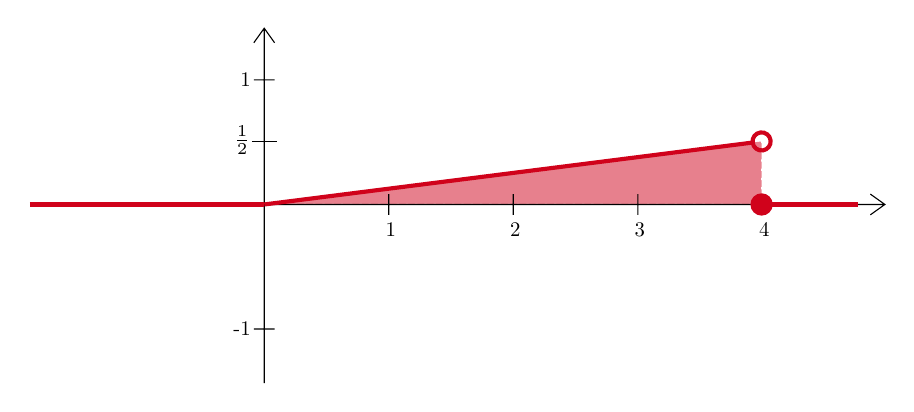
\begin{tikzpicture}[x=0.75pt,y=0.75pt,yscale=-1,xscale=1]
				%uncomment if require: \path (0,300); %set diagram left start at 0, and has height of 300
				
				%Shape: Right Triangle [id:dp3908780862434089] 
				\draw  [color={rgb, 255:red, 255; green, 255; blue, 255 }  ,draw opacity=1 ][fill={rgb, 255:red, 208; green, 2; blue, 27 }  ,fill opacity=0.5 ][dash pattern={on 0.84pt off 2.51pt}] (221,140.37) -- (460.6,110) -- (460.6,140.37) -- cycle ;
				%Shape: Axis 2D [id:dp04718372232449086] 
				\draw  (164,140.37) -- (520,140.37)(220.96,55.46) -- (220.96,226.49) (513,135.37) -- (520,140.37) -- (513,145.37) (215.96,62.46) -- (220.96,55.46) -- (225.96,62.46) (280.96,135.37) -- (280.96,145.37)(340.96,135.37) -- (340.96,145.37)(400.96,135.37) -- (400.96,145.37)(460.96,135.37) -- (460.96,145.37)(215.96,80.37) -- (225.96,80.37)(215.96,200.37) -- (225.96,200.37) ;
				\draw   (287.96,152.37) node[anchor=east, scale=0.75]{1} (347.96,152.37) node[anchor=east, scale=0.75]{2} (407.96,152.37) node[anchor=east, scale=0.75]{3} (467.96,152.37) node[anchor=east, scale=0.75]{4} (217.96,80.37) node[anchor=east, scale=0.75]{1} (217.96,200.37) node[anchor=east, scale=0.75]{-1} ;
				%Straight Lines [id:da7099499225261134] 
				\draw    (215,110) -- (227,110) ;
				%Straight Lines [id:da5425124724680095] 
				\draw [color={rgb, 255:red, 208; green, 2; blue, 27 }  ,draw opacity=1 ][line width=1.5]    (221,140.37) -- (457.27,110.42) ;
				\draw [shift={(460.6,110)}, rotate = 352.78] [color={rgb, 255:red, 208; green, 2; blue, 27 }  ,draw opacity=1 ][line width=1.5]      (0, 0) circle [x radius= 4.36, y radius= 4.36]   ;
				%Straight Lines [id:da11944528498221407] 
				\draw [color={rgb, 255:red, 208; green, 2; blue, 27 }  ,draw opacity=1 ][line width=1.5]    (108,140.37) -- (220.96,140.37) ;
				%Straight Lines [id:da6114327596724944] 
				\draw [color={rgb, 255:red, 208; green, 2; blue, 27 }  ,draw opacity=1 ][line width=1.5]    (460.6,140.37) -- (507,140.37) ;
				\draw [shift={(460.6,140.37)}, rotate = 0] [color={rgb, 255:red, 208; green, 2; blue, 27 }  ,draw opacity=1 ][fill={rgb, 255:red, 208; green, 2; blue, 27 }  ,fill opacity=1 ][line width=1.5]      (0, 0) circle [x radius= 4.36, y radius= 4.36]   ;
				
				% Text Node
				\draw (205,101.4) node [anchor=north west][inner sep=0.75pt]  [font={{\footnotesize}}]  {$\frac{1}{2}$};
				
				
				\end{tikzpicture}
				\caption{}
			\end{figure}
			\item $\dispsty\int_{1}^2\frac{1}{8}x\ dx=\frac{1}{8}\frac{1}{2}x^2\Bigg|_1^2=\frac{3}{16}$.
			\item Since \[
			EX=\int_0^4\frac{1}{8}x^2\ dx=\frac{1}{8}\frac{1}{3}x^3\Bigg|_0^4=\frac{8}{3}
			\] and \[
			E(X^2)=\int_0^4\frac{1}{8}x^3\ dx=\frac{1}{8}\frac{1}{4}x^4\Bigg|_0^4=8,
			\] we have $\Var(X)=8-\dispsty\left(\frac{8}{3}\right)^2=\frac{8}{9}$.
		\end{enumerate}
	\end{proof}
\end{example}
\
\begin{example}
	Assume that $X$ has density \[
	f_X(x)=\begin{cases}
	3x^2 &\text{if $x\in[0,1]$},\\
	0 &\text{otherwise}.
	\end{cases}
	\] Compute the density $f_Y$ of $Y=1-X^4$.\begin{proof}[\sol]
		Note that the density $f_Y(y)$ will be non-zero only when $y\in[0,1]$, as the values of $Y$ are restricted to that interval. Now, for $y\in(0,1)$, \[
		F_Y(y)=P(Y\leq y)=P(1-X^2\leq y)=P(1-y\leq X^4)=P[(1-y)^{1/4}\leq X]=\int_{(1-y)^{1/4}}^13x^2\ dx.
		\] It follows that \[
		f_Y(y)=\frac{d}{dy}F_Y(y)=\frac{d}{dy}\left[\int_{(1-y)^{1/4}}^13x^2\ dx\right]=\frac{d}{dy}\left[1-(1-y)^{3/4}\right]=-\frac{3}{4}(1-y)^{-1/4}(-1)=\frac{3}{4}\frac{1}{(1-y)^{1/4}}
		\] for $y\in(0,1)$, and $f_Y(y)=0$ otherwise. Observe that it is immaterial how $f(y)$ is defined at $y=0$ and $y=1$, because those two values contribute nothing to any integral.
	\end{proof} 
\end{example}

\newpage
\subsection{Uniform Random Variable}
Uniform random variable represents the choice of a \textbf{random number} in $[\alpha,\beta]$. For $[\alpha,\beta]=[0,1]$, this is ideally the output of a \textit{computer random number generator}.
\begin{tcolorbox}[colback=white]
	\begin{definition}
		A random variable is uniform if it has the probability density function given below. \[
		\text{Density}:\ f(x)=\begin{cases}
		\displaystyle\frac{1}{\beta-\alpha} &\text{if}\ x\in[\alpha,\beta],\\
		0 &\text{otherwise}.
		\end{cases}
		\]
	\end{definition}
\end{tcolorbox}\
\
\begin{figure}[h!]
	\centering
	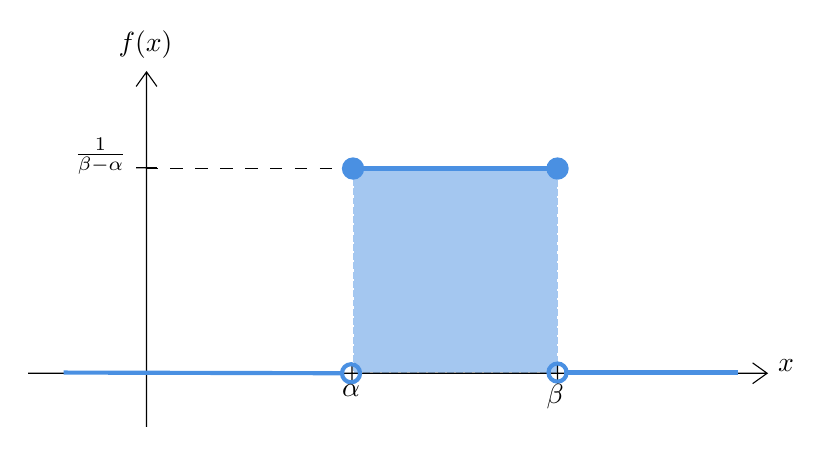
\begin{tikzpicture}[x=0.75pt,y=0.75pt,yscale=-1,xscale=1]
	%uncomment if require: \path (0,300); %set diagram left start at 0, and has height of 300
	
	%Straight Lines [id:da09412642956157424] 
	\draw  [dash pattern={on 4.5pt off 4.5pt}]  (220.5,102) -- (320.5,102) ;
	%Shape: Rectangle [id:dp1631648535679342] 
	\draw  [color={rgb, 255:red, 255; green, 255; blue, 255 }  ,draw opacity=1 ][fill={rgb, 255:red, 74; green, 144; blue, 226 }  ,fill opacity=0.5 ][dash pattern={on 0.84pt off 2.51pt}] (320.5,102) -- (419.02,102) -- (419.02,200.3) -- (320.5,200.3) -- cycle ;
	%Shape: Axis 2D [id:dp04718372232449086] 
	\draw  (164,200.64) -- (520,200.64)(221,55.46) -- (221,226.49) (513,195.64) -- (520,200.64) -- (513,205.64) (216,62.46) -- (221,55.46) -- (226,62.46) (320,195.64) -- (320,205.64)(419,195.64) -- (419,205.64)(216,101.64) -- (226,101.64) ;
	\draw   ;
	%Straight Lines [id:da21071523394189628] 
	\draw [color={rgb, 255:red, 74; green, 144; blue, 226 }  ,draw opacity=1 ][line width=1.5]    (320.5,102) -- (419.02,102) ;
	\draw [shift={(419.02,102)}, rotate = 0] [color={rgb, 255:red, 74; green, 144; blue, 226 }  ,draw opacity=1 ][fill={rgb, 255:red, 74; green, 144; blue, 226 }  ,fill opacity=1 ][line width=1.5]      (0, 0) circle [x radius= 4.36, y radius= 4.36]   ;
	\draw [shift={(320.5,102)}, rotate = 0] [color={rgb, 255:red, 74; green, 144; blue, 226 }  ,draw opacity=1 ][fill={rgb, 255:red, 74; green, 144; blue, 226 }  ,fill opacity=1 ][line width=1.5]      (0, 0) circle [x radius= 4.36, y radius= 4.36]   ;
	%Straight Lines [id:da9805578295415669] 
	\draw [color={rgb, 255:red, 74; green, 144; blue, 226 }  ,draw opacity=1 ][line width=1.5]    (181,200.3) -- (316.16,200.63) ;
	\draw [shift={(319.52,200.64)}, rotate = 0.14] [color={rgb, 255:red, 74; green, 144; blue, 226 }  ,draw opacity=1 ][line width=1.5]      (0, 0) circle [x radius= 4.36, y radius= 4.36]   ;
	%Straight Lines [id:da5823542558555885] 
	\draw [color={rgb, 255:red, 74; green, 144; blue, 226 }  ,draw opacity=1 ][line width=1.5]    (422.37,200.3) -- (506,200.3) ;
	\draw [shift={(419.02,200.3)}, rotate = 0] [color={rgb, 255:red, 74; green, 144; blue, 226 }  ,draw opacity=1 ][line width=1.5]      (0, 0) circle [x radius= 4.36, y radius= 4.36]   ;
	
	% Text Node
	\draw (524,192.7) node [anchor=north west][inner sep=0.75pt]    {$x$};
	% Text Node
	\draw (206.28,34.4) node [anchor=north west][inner sep=0.75pt]    {$f( x)$};
	% Text Node
	\draw (314,204.7) node [anchor=north west][inner sep=0.75pt]    {$\alpha $};
	% Text Node
	\draw (412.52,204.7) node [anchor=north west][inner sep=0.75pt]    {$\beta $};
	% Text Node
	\draw (185,85.9) node [anchor=north west][inner sep=0.75pt]    {$\frac{1}{\beta -\alpha }$};
	
	
	\end{tikzpicture}
	\caption{}
\end{figure}
\
\begin{tcolorbox}[colback=white]\textbf{
	Properties of Uniform Random Variable:}\begin{enumerate}
	\item $EX=\dispsty\frac{\alpha+\beta}{2}$.
	\item $\Var(X)=\dispsty\frac{(\beta-\alpha)^2}{12}$.
\end{enumerate}
\end{tcolorbox}
\begin{proof}
	\begin{enumerate}
		\item \[
		EX=\int_\alpha^\beta x\cdot\frac{1}{\beta-\alpha}\ dx=\left(\frac{1}{\beta-\alpha}\right)\frac{1}{2}x^2\Bigg|_\alpha^\beta=\frac{\beta^2-\alpha^2}{2(\beta-\alpha)}=\frac{\alpha+\beta}{2}.
		\]
		\item Note that \[
		EX^2=\int_\alpha^\beta x^2\cdot\frac{1}{\beta-\alpha}\ dx=\left(\frac{1}{\beta-\alpha}\right)\frac{1}{3}x^3\Bigg|_\alpha^\beta=\frac{\beta^3-\alpha^3}{3(\beta-\alpha)}=\frac{\alpha^2+\beta^2+\alpha\beta}{3}.
		\] Thus, \begin{align*}
		\Var(X)=EX^2-(EX)^2&=\frac{\alpha^2+\beta^2+\alpha\beta}{3}-\left(\frac{\alpha+\beta}{2}\right)^2\\
		&=\frac{\alpha^2+\beta^2+\alpha\beta}{3}-\frac{\alpha^2+\beta^2+2\alpha\beta}{4}\\
		&=\frac{4(\alpha^2+\beta^2+\alpha\beta)-3(\alpha^2+\beta^2+2\alpha\beta)}{12}\\
		&=\frac{\alpha^2+\beta^2-2\alpha\beta}{12}=\frac{(\beta-\alpha)^2}{12}.
		\end{align*}
	\end{enumerate}
\end{proof}
\begin{example}
	Assume that $X$ is uniform on $[0,1]$. (a) What is $P(X\in\mathbb{Q})$? (b) What is the probability that the binary expansion of $X$ starts with $0.010$?\begin{proof}[\sol]
		(a) As $\mathbb{Q}$ is countable, it has an enumeration, say, $\set{q_1,q_2,\cdots}$. By Axiom 3 of Probability, \[
		P(X\in\mathbb{Q})=P\left(\bigcup_{i\in I}\set{X=q_i}\right)=\sum_{i\in I}P(X=q_i)=0.
		\] Note that $P(X\in\mathbb{R})=P(\Omega)=1$.\\
		\\
		(b) As $X$ is, with probability $1$, irrational, its binary expansion is uniquely defined, so there is no ambiguity about what the second question means.\par
		Divide $[0,1)$ into $2^n$ intervals of equal length. If the binary expansion of a number $x\in[0,1)$ is $0.x_1x_2\cdots,$ the first $n$ binary digits determine which of the $2^n$ subintervals $x$ belong to: if you know that $x$ belongs to an interval $I$ based on the first $n-1$ digits, then $n$-th digit 1 means that $x$ is in in the right half of $I$ and $n$-th digit 0 means that $x$ in the left half of $I$. Thus, if the expansion starts with $0.010$, then number is in $\left[0,\frac{1}{2}\right]$, then is $\left[\frac{1}{4},\frac{1}{2}\right]$, and then finally in $\left[\frac{1}{4},\frac{3}{8}\right]$. Our answer is $1/8$.
	\end{proof}
\end{example}
\
\begin{example}
	A uniform random number $X$ divides $[0,1]$ into two segments. Let $R$ be the ratio of the smaller versus the large segment. Compute the density of $R$.	\begin{proof}[\sol]
	As $R$ has value in $(0,1)$, the density $f_R(r)$ is non-zero only for $r\in(0,1)$ and we will deal only with such $r$'s.\begin{align*}
	F_R(r)=P(R\leq r)=P\left(X\leq\frac{1}{2},\ \frac{X}{1-X}\leq r\right)+P\left(X>\frac{1}{2},\ \frac{1-X}{X}\leq r\right).
	\end{align*} Note that \begin{align*}
	\frac{X}{1-X}\leq r&\implies\frac{1-X}{X}\geq\frac{1}{r}\implies\frac{1}{X}-1\geq \frac{1}{r}\implies\frac{1}{X}\geq\frac{r+1}{r}\implies X\leq\frac{r}{r+1},\\
	\frac{1-X}{X}\leq r&\implies\frac{1}{X}-1\leq r\implies\frac{1}{X}\leq r+1\implies X\geq\frac{1}{r+1}.
	\end{align*} Thus, \begin{align*}
	F_R(r)=P(R\leq r)&=P\left(X\leq\frac{1}{2},\ X\leq \frac{r}{r+1}\right)+P\left(X>\frac{1}{2},\ X\geq\frac{1}{r+1}\right)\\
	&=P\left(X\leq\frac{r}{r+1}\right)+P\left(X\geq\frac{1}{r+1}\right)\quad\left(\because \frac{r}{r+1}\leq\frac{1}{2}\ \text{and}\ \frac{1}{r+1}\geq\frac{1}{2}\right)\\
	&=\frac{r}{r+1}+1-\frac{1}{r+1}=\frac{2r}{r+1}.
	\end{align*}
	For $r\in(0,1)$, the density, thus, equals $\dispsty
	f_R(r)=\frac{d}{dr}F_R(r)=\frac{2}{(r+1)^2}.
	$ Hence \[
	f_R(r)=\begin{cases}
	\dispsty\frac{2}{(r+1)^2} &\text{if}\ r\in(0,1),\\
	0 &\text{otherwise}.
	\end{cases}
	\]
	\end{proof}
\end{example}
\
\subsection{Exponential Random Variable}
\begin{tcolorbox}[colback=white]
	\begin{definition}
		A random variable is Exponential$(\lambda)$, with parameter $\lambda>0$, if it has the probability density function given below. \[
		\text{Density}:\ f(x)=\begin{cases}
		\lambda e^{-\lambda x} &\text{if $x\geq 0$},\\
		0 &\text{if $x<0$}.
		\end{cases}
		\]
	\end{definition}
\end{tcolorbox} This is a distribution for the \hl{\textit{waiting time}} for some random event, for example, for a lightbulb to burn out or for the next earthquake of a t lest some given magnitude.
\\
\begin{tcolorbox}[colback=white]
	\textbf{Properties of Exponential Random Variable:}\begin{enumerate}
		\item $\dispsty EX=\frac{1}{\lambda}$.
		\item $\dispsty \Var(X)=\frac{1}{\lambda^2}$.
		\item $\dispsty P(X\geq x)=e^{-\lambda x}$.
		\item Memoryless Property: $\dispsty P(X\geq x+y|X\geq y)=e^{-\lambda x}$.
	\end{enumerate}
\end{tcolorbox} The last property means that, if the event has not occurred by some given time (no matter large), the distribution of the remaining waiting time is the same as it was at the beginning. There is no ``aging''.
\begin{proof}
	Note that \[
	F_X(x)=P(X\leq x)=\int_0^x\lambda e^{-\lambda t}\ dt=1-e^{-\lambda x}.
	\] \begin{enumerate}
		\item \begin{align*}
		EX&=\int_0^\infty x\lambda e^{\lambda x}\ dx\\
		&=\frac{1}{\lambda}\int_0^\infty ye^{-y}\ dy\quad\text{where}\quad y=\lambda x\\
		&=\frac{1}{\lambda}\left[-e^{-y}-ye^{-y}\right]_0^\infty=\frac{1}{\lambda}.
		\end{align*}
		\item Since \begin{align*}
		EX^2&=\int_0^\infty x^2\lambda e^{\lambda x}\ dx\\
		&=\int_0^\infty x\cdot x\lambda e^{\lambda x}\ dx \\
		&=\frac{1}{\lambda^2}\int_0^\infty y^2e^{-y}\ dy\quad\text{where}\quad y=\lambda x\\
		&=\frac{1}{\lambda^2}\left[-2e^{-y}-2ye^{-y}-y^2e^{-y}\right]_0^\infty\\
		&=\frac{2}{\lambda^2},
		\end{align*} we obtain that $\Var(X)=EX^2-(EX)^2=\dispsty\frac{2}{\lambda^2}-\frac{1}{\lambda^2}=\frac{1}{\lambda^2}$.\\
		\item $\dispsty P(X\geq x)=1-P(X\leq x)=e^{-\lambda x}$.\\
		\item \begin{align*}
		P(X\geq x+y|X\geq y)&=\frac{P(X>x+y,X>y)}{P(X>y)}\\
		&=\frac{P(X>x+y)}{P(X>y)}\\
		&=\frac{1-F_X(x+y)}{1-F_X(y)}\\
		&=\frac{1-(1-e^{-\lambda(x+y)})}{1-(1-e^{-\lambda y})}\\
		&=\frac{e^{-\lambda(x+y)}}{e^{-\lambda y}}\\
		&=\exp\left[-\lambda(x+y)-(-\lambda y)\right]\\
		&=e^{-\lambda x}(=P(X>x)).
		\end{align*}
	\end{enumerate}
\end{proof}
\
\begin{example}
	Assume that a lightbulb lasts on average 100 hours. Assuming exponential distribution, compute the probability that it lasts more than 200 hours and the probability that it lasts less than 50 hours.
	\begin{proof}[\sol]
		Let $X$ be the waiting time for the bulb to burn out. Then, $X$ is Exponential with $\lambda=1/100\ (\because EX=1/\lambda=100)$. And then \begin{align*}
		F_X(x)=P(X\leq x)=\int_0^x\lambda e^{-\lambda t}\ dt=-e^{-\lambda t}\Bigg|_0^x=1-e^{-\lambda x},
		\end{align*} so $\dispsty
		F_X(x)\Bigg|_{\lambda=\frac{1}{100}}=1-\exp\left(-\frac{x}{100}\right)$. Thus, \begin{align*}
		P(X\geq 200)&=1-F_X(200)=e^{-2}\approx 0.1353,\\
		P(X\leq 50)&=F_X(50)=1-e^{-1/2}\approx0.3935.
		\end{align*}
	\end{proof}
\end{example}
\newpage
\subsection{Normal Random Variable}
\begin{tcolorbox}[colback=white]
	\begin{definition}
		A random variable is \textbf{Normal with parameter $\mu\in\mathbb{R}$ and $\sigma^2>0$} or, in short, \textbf{$X$ is $N(\mu,\sigma^2)$}, if its density is the function given below. \[
		\text{Density}:\ f(x)=f_X(x)=\frac{1}{\sigma\sqrt{2\pi}}\exp\left[-\frac{(x-\mu)^2}{2\sigma^2}\right],
		\] where $x\in(-\infty,\infty)$.
	\end{definition}
\end{tcolorbox} 
\
\begin{tcolorbox}[colback=white]
	\textbf{Properties of Normal Random Variable:}\begin{enumerate}
		\item For $f(x)=\dispsty\frac{1}{\sigma\sqrt{2\pi}}\exp\left[-\frac{(x-\mu)^2}{2\sigma^2}\right]$,\quad $
		\dispsty\int_{-\infty}^{\infty} f(x)\ dx=1.
		$
		\item $EX=\mu$.
		\item $\Var(X)=\sigma^2$.
	\end{enumerate}
\end{tcolorbox}
\
\begin{proof}
	\ \begin{enumerate}
		\item Let $\dispsty\frac{x-\mu}{\sigma}=t$, \ie, $\dispsty\frac{1}{\sigma}\ dx=dt$. Then \begin{align*}
		\int_{-\infty}^\infty\frac{1}{\sigma\sqrt{2\pi}}\exp\left[-\frac{(x-\mu)^2}{2\sigma^2}\right]\ dx=\frac{1}{\sqrt{2\pi}}\int_{-\infty}^\infty \exp\left(-\frac{t^2}{2}\right)\ dt.
		\end{align*} Let $\dispsty S=\int_{-\infty}^\infty e^{-ax^2}\ dx=\int_{-\infty}^\infty e^{-ay^2}\ dy$. Then \begin{align*}
		S^2=\int_{-\infty}^{\infty}\int_{-\infty}^{\infty}e^{-a(x^2+y^2)}\ dx\ dy&=\int_0^{2\pi}\int_{0}^{\infty}e^{-ar^2} r\ dr\ d\theta\\
		&=\int_0^{2\pi}-\frac{1}{2a}\left[e^{-r^2}\right]_0^\infty\ d\theta\\
		&=\left[\frac{1}{2a}\theta\right]_0^{2\pi}=\frac{\pi}{a}.
		\end{align*} Thus, $S=\dispsty\sqrt{\frac{\pi}{a}}$. Hence \[
		\frac{1}{\sqrt{2\pi}}\int_{-\infty}^\infty \exp\left(-\frac{t^2}{2}\right)\ dt=\frac{1}{\sqrt{2\pi}}\sqrt{2\pi}=1.
		\]
		\item \begin{align*}
		E(X)&=\int_{-\infty}^\infty xf(x)\ dx\\&=\int_{-\infty}^\infty x\frac{1}{\sigma\sqrt{2\pi}}\exp\left[-\frac{(x-\mu)^2}{2\sigma^2}\right]\ dx\\
		&=\int_{-\infty}^\infty \left[(x-\mu)+\mu\right]\frac{1}{\sigma\sqrt{2\pi}}\exp\left[-\frac{(x-\mu)^2}{2\sigma^2}\right]\ dx\\
		&=\int_{-\infty}^\infty (x-\mu)\frac{1}{\sigma\sqrt{2\pi}}\exp\left[-\frac{(x-\mu)^2}{2\sigma^2}\right]\ dx+\int_{-\infty}^\infty \mu\frac{1}{\sigma\sqrt{2\pi}}\exp\left[-\frac{(x-\mu)^2}{2\sigma^2}\right]\ dx\\
		&=\frac{1}{\sigma\sqrt{2\pi}}(-\sigma^2)\int_{-\infty}^\infty\frac{-x+\mu}{\sigma^2}\exp\left[-\frac{(x-\mu)^2}{2\sigma^2}\right]\ dx +\mu\int_{-\infty}^\infty\frac{1}{\sigma\sqrt{2\pi}}\exp\left[-\frac{(x-\mu)^2}{2\sigma^2}\right]\ dx\\
		&=\frac{1}{\sigma\sqrt{2\pi}}(-\sigma^2)\left[\exp\left[-\frac{(x-\mu)^2}{2\sigma^2}\right]\right]_{-\infty}^\infty+\mu\\
		&=\mu.
		\end{align*}
		\item \[
		\Var(X)=E[(X-E[X]^2)]=\int_{-\infty}^\infty(x-\mu)^2\cdot f(x)\ dx=\int_{-\infty}^\infty(x-\mu)^2\frac{1}{\sigma\sqrt{2\pi}}\exp\left[-\frac{(x-\mu)^2}{2\sigma^2}\right]\ dx.
		\] Let $\omega=\dispsty\frac{x-\mu}{\sigma\sqrt{2}}$  $\left(\text{here},\ d\omega=\dispsty\frac{1}{\sigma\sqrt{2}}dx\right)$, then \[
		\Var(X)=\int_{-\infty}^\infty\sigma^22\omega^2\frac{1}{\sigma\sqrt{2\pi}}e^{-\omega^2}\sigma\sqrt{2}\ d\omega=\frac{2\sigma^2}{\sqrt{\pi}}\int_{-\infty}^\infty\omega\cdot\omega e^{-\omega^2}\ d\omega.
		\] Using integration by parts: \begin{table}[h!]
			\centering\begin{tabular}{c|c}
				Differentiation & Integration\\
				\midrule
				$\omega$ & $\dispsty\omega e^{-\omega^2}$\\
				\hline
				$1$ & $\displaystyle -1/2e^{-\omega^2}$
			\end{tabular}
		\end{table}\ \\ we have \begin{align*}
	\Var(X)&=\frac{2\sigma^2}{\sqrt{\pi}}\left(\crossout[red]{\text{$0$ by L'H$\hat{\text{o}}$pital's rule}}{\omega\frac{-1}{2}e^{-\omega^2}\Bigg|_{-\infty}^{\infty}}-\int_{-\infty}^\infty\frac{-1}{2}e^{-\omega^2}d\omega\right)\\
	&=\frac{2\sigma^2}{\sqrt{\pi}}\left(\frac{1}{2}\int_{-\infty}^\infty e^{-\omega^2}\right)\\
	&=\frac{2\sigma^2}{\sqrt{\pi}}\cdot\frac{1}{2}\cdot\sqrt{\pi}=\sigma^2.
	\end{align*}
	\end{enumerate}
\end{proof}
\
\begin{tcolorbox}[colback=white]
	If $X\sim N(\mu_X,\sigma_X^2)$ and $Y=aX+b$ where $a,b\in\mathbb{R}$, then \[
	Y\sim N(\mu_Y, \sigma_Y^2)\quad\text{where}\quad \mu_Y=a\mu_X+b\ \text{and}\ \sigma_Y^2=a^2\sigma_X^2.
	\]\tcblower\begin{proof}
		\ \begin{itemize}
			\item $EY=E(aX+b)=aEX+b=a\mu_X+b$.
			\item $\Var(Y)=\Var(aX+b)=a^2\Var(X)=a^2\sigma_X^2$.
		\end{itemize}
	\end{proof}
\end{tcolorbox}
\
\begin{example}
	Let $X$ be a $N(\mu,\sigma^2)$ random variable and let $Y=\alpha X+\beta$, with $\alpha>0$. How is $Y$ distributed?\begin{proof}[\sol]
		From \begin{align*}
		F_Y(y)=P(Y\leq y) &=P(\alpha X+\beta\leq y)\\
		&=P\left(X\leq\frac{y-\beta}{\alpha}\right)\\
		&=\int_{-\infty}^{\dispsty\frac{y-\beta}{\alpha}}f_X(x)\ dx,
		\end{align*} we have \begin{align*}
		\frac{d}{dt}F_Y(y)=f_Y(y)&=f_X\left(\frac{y-\beta}{\alpha}\right)\cdot\frac{1}{\alpha}\\
		&=\frac{1}{\sqrt{2\pi}\sigma}\frac{1}{\alpha}\exp\left[-\frac{(y-\beta-\alpha\mu)^2}{2\alpha^2\sigma^2}\right]=\frac{1}{\sqrt{2\pi}(\alpha\sigma)}\exp\left[-\frac{(y-(\alpha\mu+\beta))^2}{2(\alpha\sigma)^2}\right].
		\end{align*} Therefore, $Y$ is normal with $EY=\alpha\mu+\beta$ and $\Var(Y)=(\alpha\sigma)^2$.
	\end{proof}
\end{example}
\
\begin{note}
	In particular, \[
	Z=\frac{X-\mu}{\sigma}=\frac{1}{\sigma}X+\left(-\frac{\mu}{\sigma}\right)
	\] has $EZ=0$ and $\Var(Z)=1$. Such a $N(0,1)$ random variable is called \textit{standard} Normal. Its distribution function $F_Z(z)$ is denoted by $\Phi(z)$. Note that \begin{align*}
	\Phi(z)=F_Z(z)&=\frac{1}{\sqrt{2\pi}}\int_{-\infty}^ze^{-x^2/2}\ dx,\\
	f_Z(z)&=\frac{1}{\sqrt{2\pi}}e^{-z^2/2}.
	\end{align*} You should also note that it is enough to know these values for $z>0$, as in this case, by using the fact that $f_Z(x)$ is an even function: \[
	\Phi(-z)=\int_{-\infty}^{-z}f_Z(x)\ dx=\int_{z}^{\infty}f_Z(x)\ dx =1-\int_{-\infty}^zf_Z(x)\ dx=1-\Phi(z).
	\] In particular, $\Phi(0)=1/2$ because $\Phi(0)=1-\Phi(0)$. Another way to write this is $P(Z\geq -z)=P(Z\leq z)$ for all $z\in\mathbb{R}$.
\end{note}
\begin{example}
	What is the probability that a Normal random variable differs from its mean $\mu$ by more than $\sigma$ More than $2\sigma$? More than $3\sigma$?\begin{proof}[\sol]
		For $X\sim N(\mu,\sigma^2)$, we need to compute \begin{align*}
		P(\abs{X-\mu}\geq\sigma),\\
		P(\abs{X-\mu}\geq2\sigma),\\
		P(\abs{X-\mu}\geq3\sigma).
		\end{align*} We have \[
		P(\abs{X-\mu}\geq\sigma)=P\left(\abs{\frac{X-\mu}{\sigma}}\geq1\right)=P(\abs{Z}\geq 1)=2P(Z\geq 1)=2(1-\Phi(1))\approx0.3713.
		\] Similarly, \begin{align*}
		P(\abs{X-\mu}\geq2\sigma)=2(1-\Phi(2))\approx0.0455,\\
		P(\abs{X-\mu}\geq3\sigma)=2(1-\Phi(3))\approx0.0027.
		\end{align*}
	\end{proof}
\end{example}
\begin{example}
	Assume that $X$ is Normal with mean $\mu=2$ and variance $\sigma^2=25$. Compute the probability that $X$ is between $1$ and $4$.\begin{proof}[\sol]
		\begin{align*}
		P(1\leq X\leq 4)=P\left(\frac{1-2}{5}\leq\frac{X-2}{5}\leq\frac{4-2}{5}\right)
		&=P(-0.2\leq Z\leq 0.4)\\
		&=P(Z\leq 0.4)-P(Z\leq -0.2)\\
		&=\Phi(0.4)-(1-\Phi(0.2))\approx0.2347.
		\end{align*}
	\end{proof}
\end{example}
\
\begin{tcolorbox}[colback=white]
	\begin{theorem}[\bf De Moivre-Laplace Central Limit Theorem]
		Let $S_n$ be $\text{Binomial(n,p)}$, where $p$ is fixed and $n$ is large. Then, $\dispsty\frac{S_n-np}{\sqrt{np(1-p)}}\approx N(0,1)$; more precisely, \[
		P\left(\frac{S_n-np}{\sqrt{np(1-p)}}\leq x\right)\to\Phi(x)
		\] as $n\to\infty$, for every real number $x$.
	\end{theorem}\tcblower
	We should also note that the above theorem is an analytical statement; it says that \[
	P\left(S_n\leq np+x\sqrt{np(1-p)}\right)=\sum_{0\leq k\leq np+x\sqrt{np(1-p)}}\binom{n}{k}p^k(1-p)^{n-k}\to\frac{1}{\sqrt{2\pi}}\int_{-\infty}^xe^{t^2/2}\ dt
	\] as $n\to\infty$, for every $x\in\mathbb{R}$.
\end{tcolorbox}
\
\begin{remark}
	Remember that, when $n$ is large and $p$ is small, say $n=100$ and $p=1/100$, the Poisson approximation (with $\lambda=np$) is much better!
\end{remark}
\begin{example}
	A roulette wheel has 38 slots: 18 red, 18 black, and 2 green. The ball ends at one of these at random. You are a player who plays a large number of games and makes an even bet of \$1 on red in every game. After $n$ games, what is the probability that you are ahead? Answer this for $n=100$ and $n=1000$.\begin{proof}[\sol]
		Let $S_n$ be the number of times you win. This is a $\text{Binomial}\left(n,\frac{9}{19}\right)$ random variable. \begin{align*}
		P(\text{ahead})&=P(\text{win more than half of the games})\\
		&=P\left(S_n>\frac{n}{2}\right)\\
		&=P\left(\frac{S_n-np}{\sqrt{np(1-p)}}>\frac{1/2n-np}{\sqrt{np(1-p)}}\right)\\
		&\approx P\left(Z>\frac{(1/2-p)\sqrt{n}}{\sqrt{p(1-p)}}\right).
		\end{align*} For $n=100$, we get \[
		P(Z>5/\sqrt{90})\approx0.2990,
		\] and for $n=1000$, we get \[
		P(Z>5/3)\approx0.0478.
		\]
	\end{proof}
\end{example}
\
\begin{example}
	What would the answer to the previous example be if the game were fair, \ie, you bet even money on the outcome of a fair coin toss each time.\begin{proof}[\sol]
		Then $p=1/2$ and \[
		P(\text{ahead})\to P(Z>0)=0.5,
		\] as $n\to\infty$.
	\end{proof}
\end{example}
\
\begin{example}
	How may times do you need to toss a fair coin to get $100$ heads with probability $0.9$.\begin{proof}[\sol]
		Let $n$ be the number of tosses that we are looking for. For $S_n$, which is $\text{Binomial}(n,1/2)$, we need to find $n$ so that \[
		P(S_n\geq 100)\approx0.9.
		\] We will use below that $n>200$, as the probability would be approximately $1/2$ for $n=200$ (see the previous example). Here is the computation: \begin{align*}
		P\left(\frac{S_n-1/2n}{1/2\sqrt{n}}\geq\frac{100-1/2n}{1/2\sqrt{n}}\right)\approx P\left(Z\geq\frac{100-1/2n}{1/2\sqrt{n}}\right)&=P\left(Z\geq\frac{200-n}{\sqrt{n}}\right)\\
		&=P\left(Z\geq-\left(\frac{n-200}{\sqrt{n}}\right)\right)\\
		&=P\left(Z\leq\frac{n-200}{\sqrt{n}}\right)\\
		&=\Phi\left(\frac{n-200}{\sqrt{n}}\right)\\
		&=0.9.
		\end{align*} According to the tables, $\Phi(1.28)\approx0.9$, thus we need to solve $\dispsty\frac{n-200}{\sqrt{n}}=1.28$, that is, \[
		n-1.28\sqrt{n}-200=0.
		\] This is a quadratic equation in $\sqrt{n}$, with the only positive solution \[
		\sqrt{n}=\frac{1.28+\sqrt{1.28^2+800}}{2}.
		\] Thus, $n=219$.
	\end{proof}
\end{example}
\newpage
\subsection{Exercises for Chapter 6}
\begin{enumerate}[\bf 1.]
	\item A random variable $X$ has the density function \[
	f(x)=\begin{cases}
	c(x+\sqrt{x}) & x\in[0,1],\\
	0 &\text{otherwise}.
	\end{cases}
	\] (a) Determine $c$. (b) Compute $E(1/X)$. (c) Determine the p. d. f. of $Y=X^2$.\\ \begin{proof}[\sol]
		\begin{enumerate}[(a)]
			\item We must find $c$ such that $\int_0^1 c(x+\sqrt{x})\ dx=1$. Then \[
			\int_0^1c(x+\sqrt{x})\ dx=c\left[\frac{1}{2}x^2+\frac{2}{3}x^{3/2}\right]_0^1=c\left(\frac{1}{2}+\frac{2}{3}\right)=c\cdot\frac{7}{6}=1.
			\] Thus, $c=6/7$.
			\item \begin{align*}
			E(1/X)=\int_0^1\frac{1}{x}\cdot f_X(x)\ dx &= \int_0^1\frac{1}{x}\cdot \frac{6}{7}\left(x+\sqrt{x}\right)\ dx\\
			&=\frac{6}{7}\int_0^1(1+x^{-1/2})\ dx\\
			&=\frac{6}{7}\left[x+2x^{1/2}\right]_0^1\\
			&=\frac{6}{7}(1+2)=\frac{18}{7}.
			\end{align*}
			\item For $y\in(0,1)$, \begin{align*}
			F_Y(y)=P(Y\leq y)=P(X^2\leq y)=P(X\leq \sqrt{y})&=\int_{0}^{\sqrt{y}}\frac{6}{7}(x+\sqrt{x})\ dx\\
			&=\frac{6}{7}\left[\frac{1}{2}x^2+\frac{2}{3}x^{3/2}\right]_0^{\sqrt{y}}\\
			&=\frac{6}{7}\left(\frac{1}{2}y+\frac{2}{3}y^{3/4}\right).
			\end{align*} It follows that \[
			f_Y(y)=\frac{d}{dy}F_Y(y)=\frac{d}{dy}\left[\frac{6}{7}\left(\frac{1}{2}y+\frac{2}{3}y^{3/4}\right)\right]=\frac{6}{7}\left(\frac{1}{2}+\frac{2}{3}\frac{3}{4}y^{-1/4}\right)=\frac{6}{7}\left(\frac{1}{2}+\frac{1}{2}y^{-1/4}\right)
			\] for $y\in(0,1)$, and $f_Y(y)=0$ otherwise; that is, \[
			f_Y(y)=\begin{cases}
			\dispsty\frac{3}{7}\left(1+y^{-1/4}\right) & y\in(0,1),\\
			\\
			0 & \text{otherwise}.
			\end{cases}
			\]
		\end{enumerate}
	\end{proof}\
	\item The density function of a random variable $X$ is given by \[
	f(x)=\begin{cases}
	a+bx & x\in[0,2],\\
	0 &\text{otherwise}.
	\end{cases}
	\] We also know that $E(X)=7/6$. (a) Compute $a$ and $b$. (b) Compute $\Var(X)$.\\ \begin{proof}[\sol]
		\begin{enumerate}[(a)]
			\item Note that \[
			\int_0^2(a+bx)\ dx=\left[ax+\frac{b}{2}x^2\right]_0^2=2a+2b=1\quad\cdots\quad(1)
			\] and that \[
			EX=\int_0^2x(a+bx)=\int_0^2(ax+bx^2)\ dx=\left[\frac{a}{2}x^2+\frac{b}{3}x^3\right]_0^2=2a+\frac{8}{3}b=\frac{7}{6}. \quad\cdots\quad(2)
			\] Doing $(2)-(1)$, we have \[
			a=b=\frac{1}{4}.
			\]
			\item Remind that $f_X(x)=\dispsty\frac{1}{4}\left(1+x\right)$ for $x\in[0,2]$ and that $EX=7/6$. Since \[
			EX^2=\int_0^2 x^2\left[\frac{1}{4}(1+x)\right]\ dx=\frac{1}{4}\int_0^2(x^2+x^3)\ dx=\frac{1}{4}\left[\frac{1}{3}x^3-\frac{1}{4}x^4\right]_0^2=\frac{1}{4}\left(\frac{8}{3}+4\right)=\frac{2}{3}+1=\frac{5}{3},
			\] we obtain \[
			\Var(X)=EX^2-(EX)^2=\frac{5}{3}-\left(\frac{7}{6}\right)^2=\frac{5}{3}-\frac{49}{36}=\frac{60-49}{36}=\frac{11}{36}.
			\]
		\end{enumerate}
	\end{proof}\
	\item After your complaint about their service, a representative of an insurance company promised to call you ``between 7 and 9 this evening. Assume that this means that the time $T$ of the call is uniformly distributed in the specified interval. \begin{enumerate}[(a)]
		\item Compute the probability that the call arrives between 8:00 and 8:20.
		\item At 8:30, the call still hasn't arrived. What is the probability that it arrives in the next 10 minutes?
		\item Assume that you know in advance that the call will last \textit{exactly} 1 hour. From 9 to 9:30, there is a game show on TV that you wanted to watch. Let $M$ be the amount of time of the show that you miss because of the call. Compute the expected value of $M$.
	\end{enumerate}\ \begin{proof}[\sol]
	\begin{enumerate}[(a)]
		\item Remind that the time $T$ is uniformly distributed in the interval 120 minutes (7 p.m.---9 p.m.); that is, $T$ is uniform on $[0,120]$. Thus, \[
		P(\text{the call arrives between 8:00 and 8:20})=\frac{1}{120}\cdot20=\frac{1}{6}\approx 0.167.
		\]
		\item \[
		{P(T\leq100|T\geq 90)}=\frac{P(T\leq100, T\geq 90)}{P(T\geq 90)}=\frac{10/120}{30/120}=\frac{1}{3}.
		\]
		\item Note that \[
		M=\begin{cases}
		0 &\text{if}\ T\in[0,60],\\
		T-60 &\text{if}\ T\in[60,90],\\
		30 &\text{if}\ T\in[90,120].
		\end{cases}
		\] Since the density of $T$ is $1/120$ for $T\in[0,120]$, \begin{align*}
		EM&=\int_{60}^{90}(t-60)\frac{1}{120}\ dt+\int_{90}^{120}30\cdot\frac{1}{120}\ dt\\
		&=\frac{1}{120}\left[\frac{1}{2}t^2-60t\Bigg|_{60}^{90}+30t\Bigg|_{90}^{120}\right]\\
		&=\frac{30}{120}\left[\frac{1}{60}t^2-2t\Bigg|_{60}^{90}+t\Bigg|_{90}^{120}\right]\\
		&=\frac{1}{4}\left(\frac{8100}{60}-180-(60-120)+30\right)\\
		&=\frac{1}{4}\left(\frac{8100}{60}-90\right)
		\end{align*}
	\end{enumerate}
	\end{proof}\
	\item Toss a fair coin twice. You win \$1 if \textit{at least one} of the two tosses comes out heads.\begin{enumerate}[(a)]
		\item Assume that you play this game 300 times. What is, approximately, the probability that you win at least \$250?
		\item Approximately how may times do you need to play so that you win at least \$250 with probability at least 0.99?
	\end{enumerate}
	\item Roll a dice $n$ times and let $M$ be the number of times you roll 6. Assume that $n$ is large. \begin{enumerate}[(a)]
		\item Compute the expectation $EM$.
		\item Write down an approximation, in terms on $n$ and $\Phi$, of the probability that $M$ differs from its expectation by less than 10\%.
		\item How large should $n$ be so that the probability in (b) is larger than 0.99?
	\end{enumerate}
\end{enumerate}

\newpage
\section{Joint Distributions and Independence}
\subsection{Discrete Case}
\begin{tcolorbox}[colback=white]
	Assume that you have a pair $(X,Y)$ of discrete random variable $X$ and $Y$. Their \textit{joint probability mass function} is given by \[
	p(x,y)=P(X=x,Y=y)
	\] so that \[
	P\left((X,Y)\in A\right)=\sum_{(X,Y)\in A}p(x,y)=\sum_{x}\sum_{y}p(x,y).
	\] The \textit{marginal probability mass function} are the p. m. f.'s of $X$ and $Y$, given by \begin{align*}
	P(X=x)&=\sum_{y}P(X=x, Y=y)=\sum_{y}p(x,y),\\
	P(Y=y)&=\sum_{x}P(X=x, Y=y)=\sum_{x}p(x,y).
	\end{align*}
\end{tcolorbox}
\
\begin{example}
	An urn has 2 red, 5 white, and 3 green balls. Select 3 balls at random and let $X$ be the number of red balls and $Y$ be the number of white balls. Determine (a) joint p.m.f. of $(X,Y)$, (b) marginal p.m.f.'s, (c) $P(X\geq Y)$, and (d) $P(X=2|X\geq Y)$.\begin{proof}[\sol]
		The joint p.m.f. is given by $P(X=x,Y=y)$ for all possible $x$ and $y$. Then \begin{table}[h!]
			\centering
			\begin{tabular}{c||c|c|c|c}
				\toprule[1.5pt]
				$y\backslash x$ & $0$ & $1$ & $2$ & $P(Y=y)$\\
				\hline\hline
				$0$&$1/{120}$& ${2\cdot3}/{120}$& $3/120$& $10/120$\\
				\hline
				$1$&$5\cdot3/120$&$2\cdot5\cdot3/120$&$5/120$& $50/120$\\
				\hline
				$2$&$10\cdot3/120$&$10\cdot2/120$&$0$& $50/120$\\
				\hline
				$3$&$10/120$&$0$&$0$&$10/120$ \\
				\hline
				$P(X=x)$&$56/120$&$56/120$&$8/120$&$1$ \\
				\bottomrule[1.5pt]
			\end{tabular}
			\caption{}
		\end{table}\ \\ The last row and column entries are the respective column and row sums and, therefore, determine the marginal p.m.f.'s. To answer (c) we merely add the relevant probabilities, \[
	P(X\geq Y)=\frac{1+6+3+30+5}{120}=\frac{3}{8},
	\] and, to answer (d), we compute \[
	\frac{P(X=2, X\geq Y)}{P(X\geq Y)}=\frac{8/120}{3/8}=\frac{8}{45}.
	\]
	\end{proof}
\end{example}
\
\begin{tcolorbox}[colback=white]
	\begin{definition}
		Two random variables $X$ and $Y$ are \textbf{independent} if \[
		P(X\in A, Y\in B)=P(X\in A)P(Y\in B)
		\] for all intervals $A$ and $B$. In the discrete case, $X$ and $Y$ are independent exactly when \[
		P(X=x,Y=y)=P(X=x)P(Y=y)
		\] for all possible values $x$ and $y$ of $X$ and $Y$, that is, the joint p.m.f. is the product of the marginal p.m.f.'s.
	\end{definition}
\end{tcolorbox}
\
\begin{example}
	In the previous example, are $X$ and $Y$ independent?\begin{proof}[\sol]
		No, the $0$'s in the table are dead giveaways. For example, $P(X=2,Y=2)$, but neither $P(X=2)$ nor $P(Y=2)$ is 0.
	\end{proof}
\end{example}
\
\begin{example}
	Most often, independence is an assumption. For example, roll a die twice and let $X$ be the number on the first roll and let $Y$ be the number on the second roll. Then, $X$ and $Y$ are independent.
\end{example}
\
\subsection{Continuous Case}
\begin{tcolorbox}[colback=white]
	We say that $(X,Y)$ is a \textit{joint density} $f(x,y)\geq 0$ so that \[
	P\left((X,Y)\in S\right)=\underset{S\ \ }{\iint}f(x,y)\ dx\ dy,
	\] where $S$ is some nice (say, open or closed) subset of $\mathbb{R}^2$.
\end{tcolorbox}
\
\begin{example}
	Let $(X,Y)$ be a random point in $S$, where $S$ is compact (that is, closed and bounded) subset of $\mathbb{R}^2$. This means that \[
	f(x,y)=\begin{cases}
	\dispsty\frac{1}{\text{Area}(S)}&\text{if $(x,y)\in S$},\\
	0&\text{otherwise.}
	\end{cases}
	\] This simplest example is a saure of side length 1 where \[
	f(x,y)=\begin{cases}
	1&\text{if $x\in[0,1]$ and $y\in[0,1]$},\\
	0&\text{otherwise}.
	\end{cases}
	\]
\end{example}
\newpage
\begin{example}
	Let \[
	f(x,y)=\begin{cases}
	cx^2y&\text{if $x^2\leq t\leq 1$},\\
	0&\text{otherwise}.
	\end{cases}
	\] Determine (a) the constant $c$, (b) $P(X\geq Y)$, (c) $P(X=Y)$, and (d) $P(X=2Y)$.\begin{proof}[\sol]
		Note that \begin{figure}[h!]
			\centering
		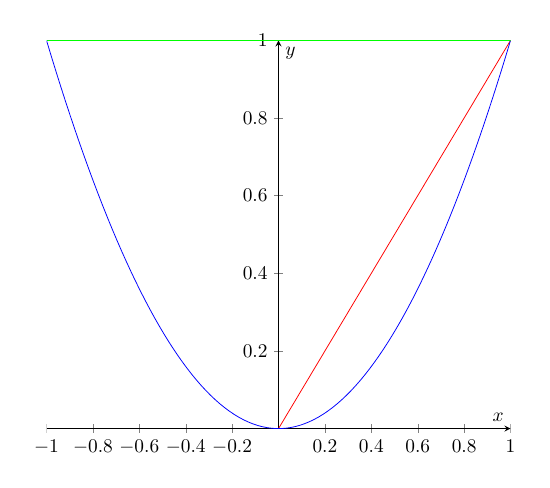
\begin{tikzpicture}[x=1pt,y=1pt,yscale=.7,xscale=.7]
		\begin{axis}[
		axis lines = center,
		xlabel = $x$,
		ylabel = {$y$},
		]
		%Below the red parabola is defined
		\addplot [
		domain=0:1,
		samples=100, 
		color=red,
		]
		{x};
%		\addlegendentry{$y=x$}
		%Here the blue parabloa is defined
		\addplot [
		domain=-1:1, 
		samples=100, 
		color=blue,
		]
		{x^2};
%		\addlegendentry{$y=x^2$}
		%Here the green parabloa is defined
		\addplot [
		domain=-1:1, 
		samples=100, 
		color=green,
		]
		{1};
%		\addlegendentry{$y=1$}
		\end{axis}
		\end{tikzpicture}
		\end{figure}\ \\ For (a), \begin{align*}
	\int_{-1}^1\int_{x^2}^1\ cx^2y\ dy\ dx&=
	\int_{-1}^1cx^2\left[\frac{1}{2}y^2\right]_{y=x^2}^{y=1}\ dx \\&=
	\int_{-1}^1\frac{cx^2}{2}(1-x^4)\ dx\\&=
	\frac{c}{2}\int_{-1}^1(x^2-x^6)\ dx\\&=
	\frac{c}{2}\left[\frac{1}{3}x^3-\frac{1}{7}x^7\right]_{-1}^1\\
	&=\frac{c}{2}\left(\frac{1}{3}-\frac{1}{7}+\left(\frac{1}{3}-\frac{1}{7}\right)\right)=c\cdot\frac{4}{21}=1,
\end{align*} and so $c=\dispsty\frac{21}{4}$. For (b), let $S$ be the region between the graphs $y=x^2$ and $y=x$, for $x\in(0,1)$. Then \begin{align*}
P(X\geq Y)=P\left((X,Y)\in S\right)&=\int_0^1\int_{x^2}^x\frac{21}{4}\cdot x^2y\ dy\ dx\\
&=\frac{21}{4}\int_0^1x^2\left[\frac{1}{2}y^2\right]_{x^2}^x\ dx\\
&=\frac{21}{8}\int_0^1x^2(x^2-x^4)\ dx\\
&=\frac{21}{8}\left[\frac{1}{5}x^5-\frac{1}{7}x^7\right]_0^1=\frac{21}{8}\cdot\frac{2}{35}=\frac{3}{20}.
\end{align*} Both probabilities in (c) and (d) are 0 because a two-dimensional integral over a line is 0.
	\end{proof}
\end{example}

\newpage
\begin{tcolorbox}[colback=white]
	If $f$ is the joint density of $(X,Y)$, then the two \textit{marginal densities}, which are the densities of $X$ and $Y$, are computed by integrating out the other variable: \begin{align*}
	f_X(x)&=\int_{-\infty}^\infty f(x,y)\ dy,\\
	f_Y(y)&=\int_{-\infty}^\infty f(x,y)\ dx.
	\end{align*}
\end{tcolorbox} Indeed, for an interval $A$, $X\in A$ means that $(X,Y)\in S$, where $S=A\times\mathbb{R}$, and, therefore, \[
P(X\in A)=\int_A\int_{-\infty}^\infty f(x,y)\ dy\ dx.
\]
\begin{tcolorbox}[colback=white]
	\begin{definition}	
	Two jointly continuous random variables $X$ and $Y$ are \textbf{independent} exactly when the joint density is the product of the marginal ones: \[
	f(x,y)=f_X(x)f_Y(y),
	\] for all $x$ and $y$.
	\end{definition}
\end{tcolorbox}
\
\begin{example}
	Previous example, continued. Compute marginal densities and determine whether $X$ and $Y$ are independent. \begin{proof}[\sol]
		We have \[
		f_X(x)=\int_{x^2}^1\frac{21}{4}\cdot x^2y\ dy=\frac{21}{8}x^2(1-x^4),
		\] for $x\in[-1,1]$, and $0$ otherwise. Moreover, \[
		f_Y(y)=\int_{-\sqrt{y}}^{\sqrt{y}}\frac{21}{4}\cdot x^2y\ dx=\frac{7}{2}y^{5/2},
		\] where $y\in[0,1]$, and $0$ otherwise. The two random variables $X$ and $Y$ are clearly not independent, as $f(x,y)\neq f_X(x)f_Y(y)$.
	\end{proof}
\end{example}
\
\begin{example}
	Let $(X,Y)$ be a random point in a square of length $1$ with the bottom left corner at the origin. Are $X$ and $Y$ independent?\begin{proof}[\sol]
		Note that \[
		f(x,y)=\begin{cases}
		1 &\text{if $(x,y)\in[0,1]\times[0,1]$},\\
		0 &\text{otherwise}.
		\end{cases}
		\] The marginal densities are \[
		\begin{cases}
		f_X(x)=1 &\text{if $x\in[0,1]$},\\
		f_Y(x)=1 &\text{if $y\in[0,1]$},\\
		0 &\text{otherwise}.
		\end{cases}
		\] Therefore, $X$ and $Y$ are independent.
	\end{proof}
\end{example}

\newpage
\begin{example}
	Let $(X,Y)$ be a random point in the triangle $\set{(x,y)\mid0\leq y\leq x\leq 1}$. Are $X$ and $Y$ independent?\begin{proof}[\sol]
		Note that \[
		f(x,y)=\begin{cases}
		2 & 0\leq y\leq x\leq 1,\\
		0 &\text{otherwise}.
		\end{cases}
		\] The marginal densities are \[
		\begin{cases}
		f_X(x)=2x &\text{if $x\in[0,1]$}\\
		f_y(x)=2(1-y) &\text{if $y\in[0,1]$}\\
		0 &\text{otherwise}.
		\end{cases}
		\] So $X$ and $Y$ are no longer distributed uniformly and no longer independent.
	\end{proof}
\end{example}
\
\begin{note}
	We can make a more general conclusion. Assume that $(X,Y)$ is a jointly continuous pair of random variables, uniform on a compact set $S\subset\mathbb{R}^2$. If they are to be independent, their marginal densities have to be constant, thus uniform on some sets, say $A$ and $B$, and then $S=A\times B$. (If $A$ and $B$ are both interval, then $S=A\times B$ is a rectangle, which is the most common example of independence.)
\end{note}
\
\begin{example}
	Mr. and Mrs. Smith agree to meet at specified location ``between 5 and 6 p.m.'' Assume that they both arrive there at a random time between 5 and 6 and that their arrivals are independent. (a) Find the density for the time one of them will have to wait for the other. (b) Mrs. Smith later tells you she had to wait; given this information, compute the probability that Mr. Smith arrived before 5:30.\begin{proof}[\sol]
		Let $X$ be the time when Mr. Smith arrives and let $Y$ be the time when Mrs. Smith arrives, with the time unit 1 hour. The assumptions imply that $(X,Y)$ is uniform on $[0,1]\times[0,1]$. For (a), let $T=\abs{X-Y}$, which has possible values in $[0,1]$. So fix $t\in[0,1]$ and compute \begin{align*}
		P(T\le t)&=P(\abs{X-Y}\leq t)\\
		&=P(-t\leq X-Y\leq t)\\
		&=P(X-t\leq Y\leq X+t)\\
		&=1-(t-t)^2\\
		&=2t-t^2,
		\end{align*} and so $f_T(t)=2-2t$. For (b), \[
		P(X\leq 0.5\mid X>Y)=\frac{P(X\leq 0.5, X>Y)}{P(X>Y)}=\frac{1/8}{1/2}=\frac{1}{4}.
		\]
	\end{proof}
\end{example}
\
\begin{example}
	Assume that $X$ and $Y$ are independent, that $X$ is uniform on $[0,1]$, and that $Y$ has density $f_Y(y)=2y$, for $y\in[0,1]$, and $0$ elsewhere. Compute $P(X+Y\leq 1)$.\begin{proof}[\sol]
		The assumptions determine the joint density of $(X,Y)$: \[
		f_X(x)f_Y(y)=f(x,y)=\begin{cases}
		2y &\text{if $(x,y)\in[0,1]\times[0,1]$}\\
		0 &\text{otherwise}.
		\end{cases}
		\] Then \[
		P(X+Y\leq 1)=\iint_0^1\int_0^{1-x}2y\ dy\ dx=\frac{1}{3},
		\] or \[
		P(X+Y\leq 1)=\iint_0^1\int_0^{1-y}2y\ dx\ dy=\frac{1}{3}.
		\] Thus, the answer is $1/3$.
	\end{proof}
\end{example}
\
\begin{example}
	Assume that you are waiting for two phone calls, from Alice and from Bob. The waiting time $T_1$ for Alice's call has expectation 10 minutes and the waiting time $T_2$ for Bob's call has expectation 40 minutes. Assume $T_1$ and $T_2$ are independent exponential random variables. What is the probability that Alice's call will come first?\begin{proof}[\sol]
		We need to compute $P(T_1<T_2)$. Assuming our unit is 10 minutes, we have, for $t_1,t_2>0$, \[
		f_{T_1}(t_1)=e^{-t_1}\quad\text{and}\quad f_{T_2}(t_2)=\frac{1}{4}e^{-t_2/4},
		\] so that the joint density is $f(t_1,t_2)=\dispsty\frac{1}{4}e^{-t_1-t_2/4}$, for $t_1,t_2\geq 0$. Therefore \begin{align*}
		P(T_1<T_2)&=\int_0^\infty\int_{t_1}^\infty\frac{1}{4}\exp\left(-t_1-\frac{t_2}{4}\right)\ dt_2\ dt_1\\
		&=\int_0^\infty\exp\left(-\frac{5t_1}{4}\right)\ dt_1\\
		&=\frac{4}{5}.
		\end{align*}
	\end{proof}
\end{example}
\
\begin{example}[\it Buffon Needle Problem]
	Parallel lines at a distinct 1 are drawn on a large sheet of paper. Drop a needle of length $l$ onto the sheet. Compute the probability that it intersects one of the lines. \begin{proof}[\sol]
		Let $D$ be the distance from the center of the needle to the nearest line and let $\Theta$ be the acute angle relative to the lines. We will, reasonably, \textit{assume} that $D$ and $\Theta$ are independent and uniform on their respective intervals $\dispsty 0\leq D\leq 1/2$ and $0\leq\Theta\leq\frac{\pi}{2}$. Then \[
		f_{D,\Theta}(d,\theta)=f_D(d)\cdot f_{\Theta}(\theta)=\frac{4}{\pi},
		\] for $(d,\theta)\in S$. And then \begin{align*}
		&\begin{cases}
		f_D(d)=2 &0\leq d\leq1/2,\\
		f_D(d)=0 &\text{otherwise}.\\
		\end{cases}\\
		&\begin{cases}
		f_\Theta(\theta)={2}/{\pi} &0\leq \theta\leq\pi/2,\\
		f_\Theta(\theta)=0 &\text{otherwise}.\\
		\end{cases}
		\end{align*} Thus, \[
		P(\text{the needle intersects a line})=P\left(D<\frac{l}{2}\sin\Theta\right).
		\]\begin{itemize}
			\item Case I: $l\leq 1$. Then, the probability equals \[
			P\left(D<\frac{l}{2}\sin\Theta\right)=\int_0^{\pi/2}\int_0^{1/2\sin\theta}\frac{4}{\pi}\ dD\ d\theta=\frac{4}{\pi}\int_0^{\pi/2}\frac{l}{2}\sin\theta\ d\theta=\frac{4}{4\pi}\cdot\frac{l}{2}=\frac{2l}{\pi}.
			\] When $l=1$, you famously get $\dispsty\frac{2}{\pi}$, which can be used to get (very poor) approximations for $\pi$.\\
			\item Case II: $l>1$. Now, the curved $d=\dispsty\frac{l}{2}\sin\theta$ intersects $d=1/2$ at $\theta=\arcsin\dispsty\frac{1}{l}$. The probability equals \[
			\frac{4}{\pi}\left[\frac{l}{2}\int_0^{\arcsin\frac{1}{l}}\sin\theta\ d\theta+\left(\frac{\pi}{2}-\arcsin\frac{1}{l}\right)\cdot\frac{1}{2}\right]=\frac{4}{\pi}\left[\frac{l}{2}-\frac{1}{2}\sqrt{l^2+1}+\frac{\pi}{4}-\frac{1}{2}\arcsin\frac{1}{l}\right].
			\]
	\end{itemize}
	\end{proof}
\end{example}
\
\begin{example}
	Assume $X_1, X_2, X_3$ are uniform on $[0,1]$ and independent. What is $P(X_1+X_2+X_3\leq 1)$?\begin{proof}[\sol]
		The joint density is \[
		f_{X_1,X_2,X_3}(x_1,x_2,x_3)=f_{X_1}(x_1)f_{Y_1}(y_1)f_{Z_1}(z_1)=\begin{cases}
		1 &\text{if $(x_1,x_2,x_3)\in[0,1]^3$},\\
		0 &\text{otherwise}.
		\end{cases}
		\] Here is how we get the answer: \[
		P(X_1+X_2+X_3\leq 1)=\int_0^1\int_0^{1-x_1}\int_0^{1-x_1-x_2}\ dx_3\ dx_2\ dx_1=\frac{1}{6}.
		\] In general, if $X_1,\dots, X_n$ are independent and uniform on $[0,1]$, \[
		P(X_1+\dots+X_n\leq 1)=\frac{1}{n!}.
		\]
	\end{proof}
\end{example}
\
\subsection{Conditional Distributions}
The conditional p. m. f. of $X$ given $Y=y$ is, in the discrete case, given simply by \[
p_X(x|Y=y)=P(X=x|Y=y)=\frac{P(X=x,Y=y)}{P(Y=y)}.
\] This is trickier in the continuous case, as we cannot divide by $P(Y=y)=0$.
\\
\begin{tcolorbox}[colback=white]
	\begin{definition}
		For a jointly continuous pair of random variables $X$ and $Y$, we define the \textit{conditional density of $X$ given $Y=y$} as follows: \[
		f_X(x|Y=y)=\frac{f(x,y)}{f_Y(y)},
		\] where $f(x,y)$ is, of course, the joint density of $(X,Y)$.
	\end{definition}
\end{tcolorbox} Observe that when $f_Y(y)=0$, $\dispsty\int_{-\infty}^\infty f(x,y)\ dx =0$, and so $f(x,y)=0$ for every $x$. So we have a $\dispsty\frac{0}{0}$ expression, which we define to be 0.\begin{quote}
	Here is a ``physicist's proof'' why this should be the conditional density formula: \begin{align*}
	P(X=x+dx|Y=y+dy)=\frac{P(X=x+dx, Y=y+dy)}{P(Y=y+dy)}&\approx\frac{f(x,y)\ dx\ dy}{f_Y(y)\ dy}\\
	&=\frac{f(x,y)}{f_Y(y)}\ dx\\
	&=f_X(x|Y=y)\ dx.
	\end{align*}
\end{quote}
\
\begin{example}
	Let $(X,Y)$ be a random point in the triangle $\set{(x,y)\mid x,y\geq 0, x+y\leq 1}$. Compute $f_X(x|Y=y)$. \begin{proof}[\sol]
		The joint density $f(x,y)$ equals 2 on the triangle. For a given $y\in[0,1]$, we know that, if $Y=y$, $X$ is between 0 and $1-y$. Moreover, \[
		f_Y(y)=\int_0^{1-y}2\ dx=2(1-y).
		\] Therefore, \[
		f_X(x|Y=y)=\begin{cases}
		\dispsty\frac{1}{1-y} &0\leq x\leq 1-y.\\
		\\
		0 &\text{otherwise}.
		\end{cases}
		\] In other words, given $Y=y$, $X$ is distributed uniformly on $[0,1-y]$, which is hardly surprising.
	\end{proof}
\end{example}
\
\begin{example}
	Suppose $(X,Y)$ has joint density \[
	f(x,y)=\begin{cases}
	\dispsty\frac{21}{4}x^2y & x^2\leq y\leq 1,\\
	\\
	0 & \text{otherwise}.
	\end{cases}
	\] Compute $f_X(x|Y=y)$. \begin{proof}[\sol]
		We compute first \[
		f_Y(y)=\frac{21}{4}y\int_{-\sqrt{y}}^{\sqrt{y}}x^2\ dx=\frac{7}{2}y^{5/2}.
		\] for $y\in[0,1]$. Then \[
		f_X(x|Y=y)=\frac{\frac{21}{4}x^2y}{\frac{7}{5}y^{5/2}}=\frac{3}{2}x^2y^{-3/2},
		\] where $-\sqrt{y}\leq x\leq\sqrt{y}$. Suppose we are asked to compute $P(X\geq Y| Y=y)$. This makes no literal sense because the probability $P(Y=y)$ of the condition is 0. We reinterpret this expression as \[
		P(X\geq y|Y=y)=\int_y^{\infty}f_X(x|Y=y)\ dx (\text{$y$ fixed}),
		\] which equals \[
		\int_y^{\sqrt{y}}\frac{3}{2}x^2y^{-3/2}\ dx=\frac{1}{2}y^{-3/2}\left(y^{3/2}-y^3\right)=\frac{1}{2}(1-y^{3/2}).
		\]
	\end{proof}
\end{example}

\section{Properties of Expectation and Variance}
\begin{center}
	\begin{tabular}{c|c|c|c|c}
		\toprule[1.5pt]
		\textbf{The Proba. Distribution} & \textbf{Parameter} & \textbf{Prob. Distribution Function} & \textbf{Mean} & \textbf{Variance} \\
		\midrule
		Binomial Distribution & $(n,p)$ & $\Pr(X=k)=\dispsty\binom{n}{k}p^k(1-p)^{n-k}$ & $np$ & $np(1-p)$\\
		\hline
		Geometric Distribution & $(p)$ & $\Pr(X=k)=(1-p)^{k-1}p$ & $\dispsty\frac{1}{p}$ & $\dispsty\frac{(1-p)}{p^2}$\\
		\hline
		Normal Distribution & $(\mu,\sigma^2)$ & $\dispsty f(x|\mu,\sigma^2)=\frac{1}{\sqrt{2\pi\sigma^2}}\exp\left(-\frac{(x-\mu)^2}{2\sigma^2}\right)$ & $\mu$ & $\sigma^2$\\
		\hline
		Uniform Distribution & $(a,b)$ & $f(x|a,b)=\begin{cases}
		\dispsty\frac{1}{b-a} & a\leq x\leq b,\\
		0 & x<a\ \text{or}\ x>b
		\end{cases}$ & $\dispsty\frac{a+b}{2}$ & $\dispsty\frac{(b-a)^2}{12}$\\
		\hline
		Exponential Distribution & $(\lambda)$ & $f(x|\lambda)=\lambda e^{-\lambda x}$ & $\dispsty\frac{1}{\lambda}$ & $\dispsty\frac{1}{\lambda^2}$\\
		\hline
		Poisson Distribution & $(\lambda)$ & $f(k|\lambda)=\dispsty\frac{e^{-\lambda}\lambda^k}{k!}$ & $\lambda$ & $\lambda$\\
		\bottomrule[1.5pt]
\end{tabular}
\end{center}
\
\subsection{Expectations}
\begin{tcolorbox}[colback=white]
	\begin{definition}
	Given a pair of random variables $(X,Y)$ with joint density $f$ and another function $g$ of two variables, \[
	E_g(X,Y)=\iint g(x,y)f(x,y)\ dx\ dy;
	\] if instead $(X,Y)$ is a discrete pair with joint probability mass function $p$, then \[
	E_g(X,Y)=\sum_{x,y}g(x,y)p(x,y).
	\]
	\end{definition}
\end{tcolorbox}
\begin{example}
	Assume that two among the 5 items are defective. Put the items in a random order and inspect them one by one. Let $X$ be the number of inspections needed to find the first defective item and $Y$ the number of additional inspections needed to find the second defective item. Compute $E\abs{X-Y}$.\begin{proof}[\sol]
		The joint p. m. f. of $(X,Y)$ is given by the following table, which lists $P(X=i, Y=j)$, together with $\abs{i-j}$ in parentheses, whenever the probability is non-zero: \begin{align*}
		P(X=1,Y=1)=P(X=1)P(Y=1|X=1)=\frac{2}{5}\cdot\frac{1}{4}=\frac{1}{10},\\
		P(X=1,Y=2)=P(X=1)P(Y=2|X=1)=\frac{2}{5}\cdot\frac{3}{4}\cdot\frac{1}{3}=\frac{1}{10}.
		\end{align*}\ \begin{center}
			\begin{tabular}{c|c|c|c|c}
				\toprule[1.5pt]
				$i\backslash j$ & 1 & 2 & 3 & 4\\
				\midrule
				$1$ & $.1 (0)$ & $.1 (1)$ & $.1 (2)$ & $.1 (3)$\\
				\hline
				$2$ & $.1 (1)$ & $.1 (0)$ & $.1 (1)$ & $0$\\
				\hline
				$3$ & $.1 (2)$ & $.1 (1)$ & $0$ & $0$\\
				\hline
				$4$ & $.1 (3)$ & $0$ & $0$ & $0$\\
				\bottomrule[1.5pt]
			\end{tabular}
		\end{center}\ \\ The answer is, therefore, $E\abs{X-Y}=1.4$.
	\end{proof}
\end{example}
\
\begin{example}
	Assume that $(X,Y)$ is a random point in the right triangle $\set{(x,y)\mid x,y\geq 0, x+y\leq 1}$. Compute $EX, EY$, and $EXY$.\begin{proof}[\sol]
		Note that the density is $2$ on the triangle, and so, \begin{align*}
		EX&=\int_0^1\int_0^{1-x}x2\ dy\ dx\\
		&=\int_0^12x(1-x)\ dx\\
		&=\frac{1}{3},
		\end{align*} and, therefore, by symmetry, $EY=EX=1/3$. And \begin{align*}
		E(XY)&=\int_0^1\int_0^{1-x}xy2\ dy\ dx\\
		&=\int_0^12x\frac{(1-x)^2}{2}\ dx\\
		&=\frac{1}{12}.
		\end{align*}
	\end{proof}
\end{example}
\subsection{Linearity and Monotonicity of Expectation}
\begin{tcolorbox}[colback=white]
	\begin{theorem}
		Expectation is linear and monotone:\begin{enumerate}
			\item For constants $a$ and $b$, $E(aX+b)=aE(X)+b$.
			\item For arbitrary random variables $X_1,\dots, X_n$ whose expected values exists, \[
			E(X_1+\cdots+X_n)=E(X_1)+\cdots+E(X_n).
			\]
			\item For two random variables $X\leq Y$, we have $EX\leq EY$.
		\end{enumerate}
	\end{theorem}\tcblower\begin{proof}
	2. We will check the second property for $n=2$ and the continuous. \[
	E(X+Y)=\iint(x+y)f(x,y)\ dx\ dy=\iint x f(x,y)\ dx\ dy+\iint yf(x,y)\ dx\ dy=EX+EY.
	\] 3. Note that $Z\geq 0\implies EZ\geq 0$. Let $Z=Y-X$, then it is proved.
\end{proof}
\end{tcolorbox}
\
\begin{note}
	We emphasize again that linearity holds for arbitrary random variables which \textit{do not need to be independent}! This is very useful. For example. we can often write a random variable $X$ as a sum of (possibly dependent) indicators, $X=I_1+\cdots+I_n$. An instance of this method is called the \textit{indicator trick}.
\end{note}
\newpage
\begin{example}
	Assume that an urn contains 10 black, 7 red, and 5 white balls. Select 5 balls (a) with and (b) without replacement and let $X$ be the number of red balls selected. Compute $EX$.\begin{proof}[\sol]
		Let $I_i$ be the indicator of the event that the $i$-th ball is red, that is, \[
		I_i=I_{\text{$i$-th ball is red}}=\begin{cases}
		1 &\text{if $i$-th ball is red},\\
		0 &\text{otherwise}.
		\end{cases}
		\] In both cases, $X=\sum_{i=1}^{5}I_i$.\begin{enumerate}
			\item In (a), $X$ is Binomial$\left(5,\frac{7}{22}\right)$, so we know that $EX=5\cdot 7/22$, but we will not use this knowledge. Instead, it is clear that \[
			EI_1=1\cdot P(\text{1st ball is red})=\frac{7}{22}=EI_2=\dots=EI_5.
			\] Therefore, by additivity, $EX=5\cdot7/22$.
			\item For (b), one solution is to compute the p. m. f. of $X$, \[
			P(X=i)=\frac{\binom{7}{i}\binom{15}{15-i}}{\binom{22}{5}},
			\] where $i=0,1,\dots,5$, and then \[
			EX=\sum_{i=0}^5i\frac{\binom{7}{i}\binom{15}{5-i}}{\binom{22}{5}}.
			\] However, the indicator trick \textit{works exactly as before}. (the fact that $I_i$ are now dependent does not matter) and so the answer is also exactly the same, $EX=5\cdot 7/22$.
		\end{enumerate}
	\end{proof}
\end{example}
\
\begin{example}[\bf Matching Problem - revisited]
	Assume that $n$ people buy $n$ gifts, which are then assigned at random, and let $X$ be the number of people who receive their own gift. What is $EX$?\begin{proof}[\sol]
		This is another problem very well suited for the indicator trick. Let $I_i=I_{\text{person}\ i\ \text{receives own gift}}$. Then, $X=\sum_{i=1}^nI_i$. Moreover, $EI_i=1/n$, for all $i$, and so $EX=1$.
	\end{proof}
\end{example}
\
\begin{example}
	Five married couples are seated around a table at random. Let $X$ be the number of wives who sit next to their husbands. What is $EX$?\begin{proof}[\sol]
		Now, let $I_i=I_{A_i}$, where $A_i=\set{\text{wife}\ i\ \text{sits next to her husband}}$ such that $P(A_i)=(8!\cdot2!)/9!$. Then, $X=\sum_{i=1}^5I_i$, and $EI_i=2/9$, so that $EX=10/9$.
	\end{proof}
\end{example}
\begin{tcolorbox}[colback=white]
	
\end{tcolorbox}
\
\begin{tcolorbox}[colback=white]
	
\end{tcolorbox}



\end{document}